\documentclass[oneside]{book}

\usepackage[left=2cm,right=2cm,top=2cm,bottom=2cm]{geometry} 

\usepackage[utf8]{inputenc}   % otra alternativa para los caracteres acentuados y la "ñ"
\usepackage[           spanish % para poder usar el español
                      ,es-tabla % para los captions de las tablas
                       ]{babel}   
\decimalpoint %para usar el punto decimal en vez de coma para los números con decimales

%\usepackage{beton}
%\usepackage[T1]{fontenc}

\usepackage{parskip}
\usepackage{xcolor}

\usepackage{caption}

\usepackage{enumerate} % paquete para poder personalizar fácilmente la apariencia de las listas enumerativas

\usepackage{graphicx} % figuras
\usepackage{subfigure} % subfiguras

\usepackage{amsfonts}
\usepackage{amsmath}

\usepackage{listings}
\lstset
{ %Formatting for code in appendix
    language=python,
    basicstyle=\footnotesize,
    stepnumber=1,
    showstringspaces=false,
    tabsize=1,
    breaklines=true,
    breakatwhitespace=false,
}

\definecolor{gris}{RGB}{220,220,220}
	
\usepackage{float} % para controlar la situación de los entornos flotantes

\restylefloat{figure}
\restylefloat{table} 
\setlength{\parindent}{0mm}


\usepackage[bookmarks=true,
            bookmarksnumbered=false, % true means bookmarks in 
                                     % left window are numbered
            bookmarksopen=false,     % true means only level 1
                                     % are displayed.
            colorlinks=true,
            allcolors=blue,
            urlcolor=blue]{hyperref}
\definecolor{webblue}{rgb}{0, 0, 0.5}  % less intense blue

\renewcommand{\thesection}{\arabic{section}}

\title{\Huge Inteligencia de Negocio: Práctica 2 \\ Visualización y Segmentación\vspace{10mm}}

\author{\huge David Cabezas Berrido \vspace{10mm} \\ 
  \huge Grupo 2: Viernes \vspace{10mm} \\ \huge dxabezas@correo.ugr.es \vspace{10mm}}

\begin{document}
\maketitle
\tableofcontents
\begin{center}
\vspace*{8cm}
\part{\textbf{Visualización}}
\end{center}

Sobre los resultados de la práctica 1, realizaremos representaciones
de los resultados obtenidos por cada algoritmo y preprocesamiento,
también de las relaciones entre los atributos. No nos centraremos en
por qué unos modelos o preprocesamientos son mejores que otros, ni en
detalles de los mismos (hiperparámetros configurados o por
defecto. Eso ya lo hicimos en la práctica anterior. Nos centraremos
cómo podemos interpretar las visualizaciones para ayudarnos a
distinguir qué algoritmo o procesamiento es más adecuado en cada caso,
o qué relaciones hay entre los atributos.

\section{Visualización de medidas}
Compararemos los scores de todos los modelos para cada
preprocesamiento y viceversa. Las métricas que representaremos son la
Accuracy y el F1-score.

\subsection{Por procesamiento}

El \textbf{primer procesamiento} consiste en \textbf{eliminar las
  instancias con valores perdidos}.

\begin{figure}[H]
  \centering
  \caption{Desempeño de los algoritmos sobre el preprocesado 1: Eliminación de valores perdidos}
  \label{fig:dropna}
  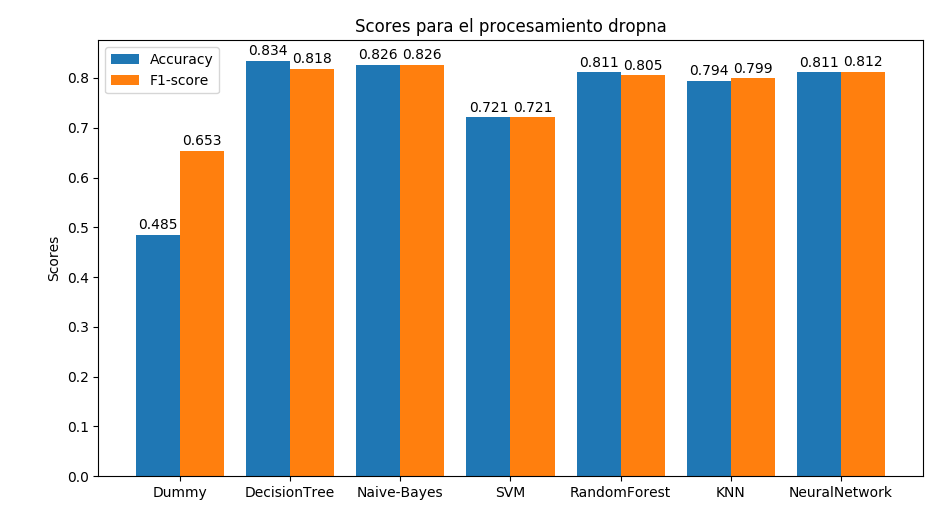
\includegraphics[width=180mm]{figures/visualizacion/dropna}
\end{figure}

La barra azul (Accuracy) representa el desempeño general del modelo,
la proporción de instancias bien clasificadas en validación
cruzada. Mientras que la barra naranja (F1-score) le da una mayor
prioridad a la clasificación de instancias positivas, que tienen mayor
importancia en este problema, puesto que un falso negativo es más
grave que un falso positivo.

Los modelos que más score han obtenido para este preprocesamiento son
el Árbol de Decisión y Naive-Bayes. El Árbol de Decisión tiene
ligeramente mayor Accuracy, mientras que Naive-Bayes tiene más
F1-score, esto significa que Decision Tree clasifica mejor las
instancias negativas que Naive-Bayes, y éste último clasifica mejor
las positivas.

SVM presenta resultados bastante peores al resto de algoritmos
(obviando Dummy).

Generalmente, la Accuracy y la F1-score son similares. La excepción es
Dummy, que clasifica bien todas las positivas pero ninguna negativa.

El \textbf{segundo procesamiento} consiste en \textbf{imputar los
  valores perdidos}, para las variables numéricas usamos la mediana y
para las nominales, la moda.

\begin{figure}[H]
  \centering
  \caption{Desempeño de los algoritmos sobre el preprocesado 2: Imputación de valores perdidos}
  \label{fig:median}
  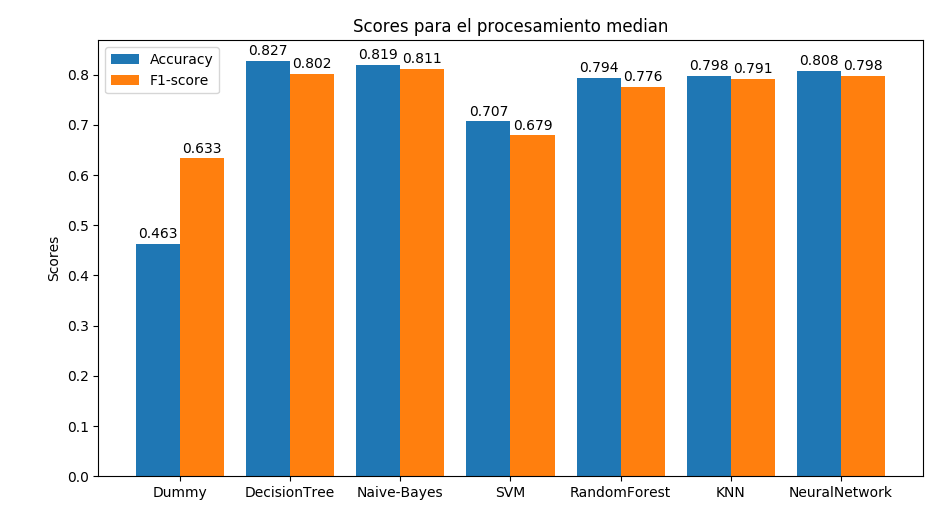
\includegraphics[width=170mm]{figures/visualizacion/median}
\end{figure}

La comparación entre los modelos no ha cambiado mucho, salvo un
descenso en el desempeño de todos los modelos. La gráfica nos ayuda a
observar, comparando las barras azules con las naranjas, que el
descenso ha sido mayor en la F1-score (la barra naranja ahora está más
abajo que la azul en todos los algoritmos salvo Dummy), esto significa
que, en general, ha empeorado la clasificación de instancias
positivas.

El \textbf{tercer procesamiento} consiste en \textbf{simplificar el
  conjunto de atributos}. Concretamente, eliminamos Density y
simplificamos la distribución de BI-Rads para que sólo tome los
valores 4 y 5.

\begin{figure}[H]
  \centering
  \label{fig:features}
  \caption{Desempeño de los algoritmos sobre el preprocesado 3: Eliminación de características innecesarias}
  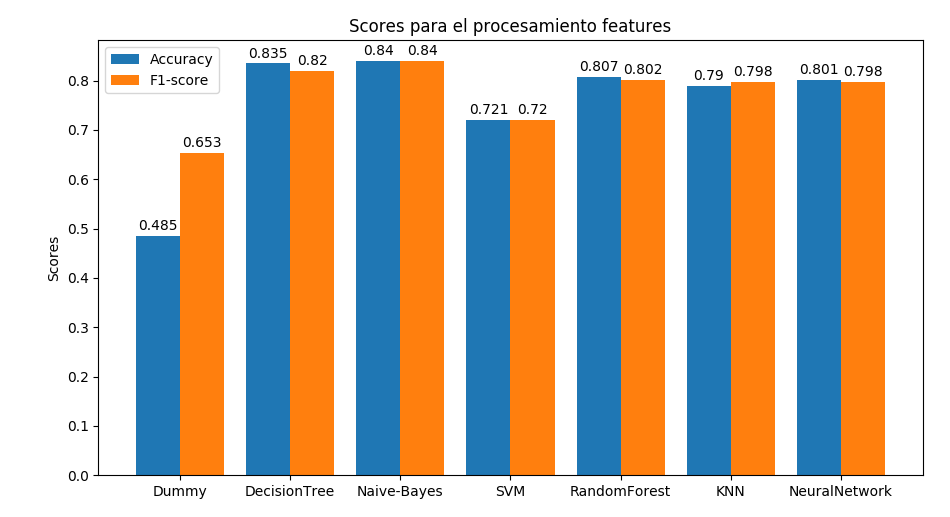
\includegraphics[width=170mm]{figures/visualizacion/features}
\end{figure}

Con este preprocesamiento, observamos que se ha recuperado la
similitud entre los valores de F1-score y Accuracy, puesto que se hizo
sobre los datos del preprocesado 1 y no sobre los del 2. También se ha
producido una mejora general en la mayoría de modelos, sobre todo en
Naive-Bayes por lo que comentamos en la práctica anterior de que
supone los atributos independientes. Sin embargo, la comparación entre
los modelos no cambia demasiado.

El \textbf{cuarto procesamiento} consiste en \textbf{binarizar las
  características nominales}, Shape y Margin. Esto lo hicimos porque
no tenía sentido medir la distancia entre valores de una variable
nominal si los numerábamos con números naturales, y algoritmos que no
tratan bien las variables nominales como KNN y Neural Network podían
verse afectados por esto.

\begin{figure}[H]
  \centering
  \label{fig:binarization}
  \caption{Desempeño de los algoritmos sobre el preprocesado 4: Binarización de características nominales}
  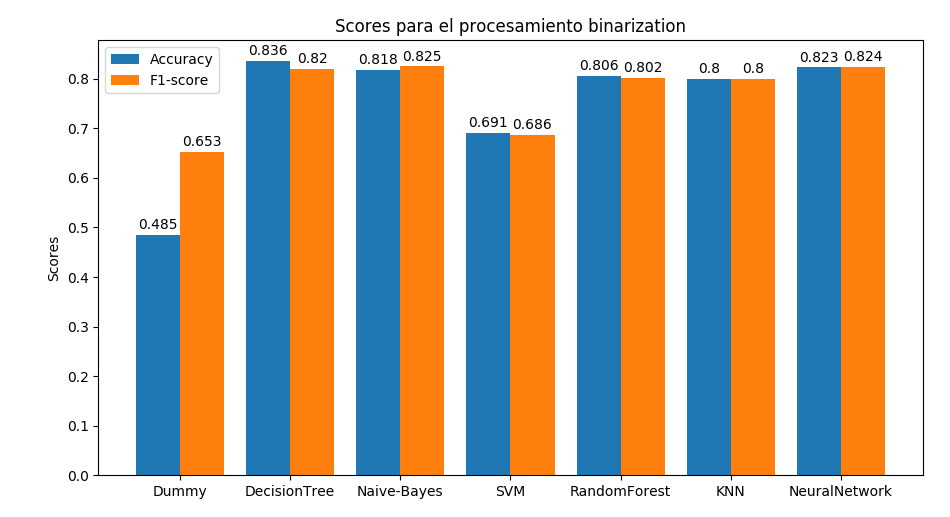
\includegraphics[width=180mm]{figures/visualizacion/binarization}
\end{figure}

Se aprecia un descenso en Naive-Bayes, por haber introducido nuevas
características que no son independientes unas de otras (cuando una
vale 1, el resto de características binarizas asociadas a la misma
variable nominal están forzadas a valer 0). La mejora en KNN es muy
leve, pero sí destaca ahora una subida en la colummna de Neural
Network.

Este procesamiento también perjudica aún más a SVM, aumenta más la
diferencia entre su columna y el resto.

El \textbf{quinto procesamiento} consiste en \textbf{reescalar las
  variables}, para que tengan media 0 y varianza 1. Esto se hizo para
solucionar la importancia exagerada que cobraba la variable Age en
algoritmos como KNN.

\begin{figure}[H]
  \centering
  \label{fig:stdScaler}
  \caption{Desempeño de los algoritmos sobre el preprocesado 5: Estandarizado de los datos}
  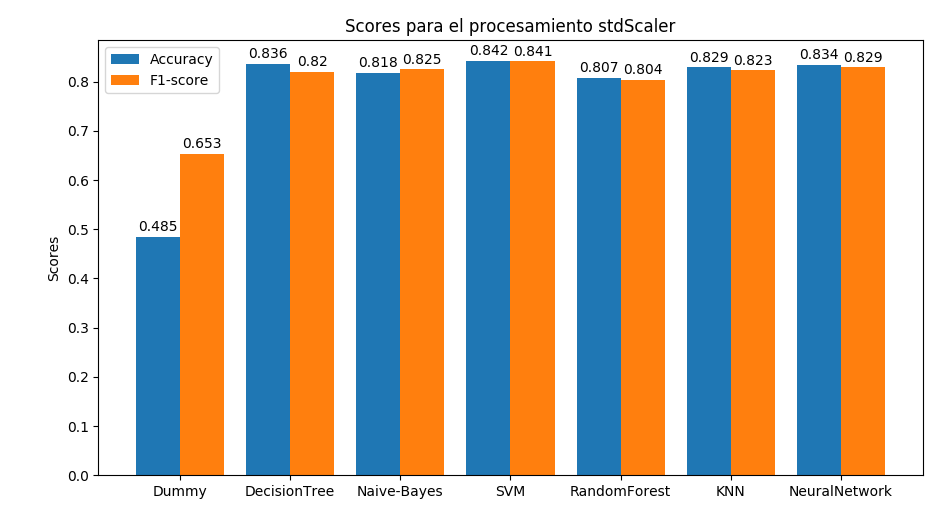
\includegraphics[width=180mm]{figures/visualizacion/stdScaler}
\end{figure}

Lo que más descata en esta gráfica es la importante subida de SVM, su
columna sube hasta acabar ligeramente por encima del resto. También
observamos una subida notable en el desempeño de KNN, cuya barra
adelanta a la de Random Forest.

\subsection{Por modelo}

\begin{figure}[H]
  \centering
  \label{fig:dummy}
  \caption{Desempeño de Dummy para cada preprocesamiento}
  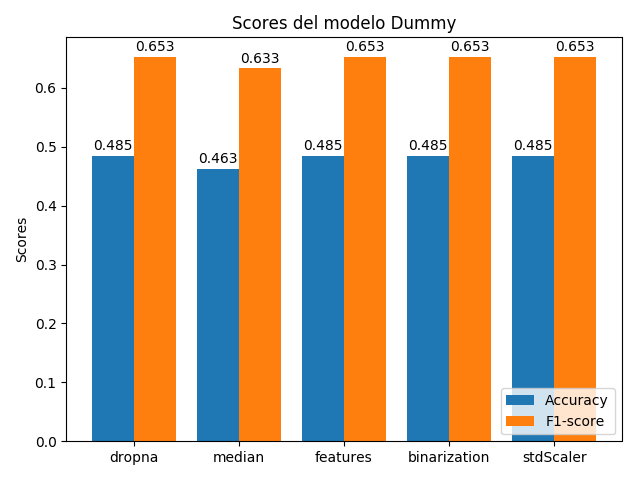
\includegraphics[width=90mm]{figures/visualizacion/dummy}
\end{figure}

No hay mucho que comentar de Dummy, consigue los mismos scores para
todos los preprocesamientos, ya que ignora los datos de entrada y se
limita a predecir siempre maligno. Cambia para el el segundo
preprocesamiento, porque varía el número de instancias, ya que no
eliminamos las instancias con valores perdidos.

\begin{figure}[H]
  \centering
  \label{fig:dt}
  \caption{Desempeño de Decision Tree para cada preprocesamiento}
  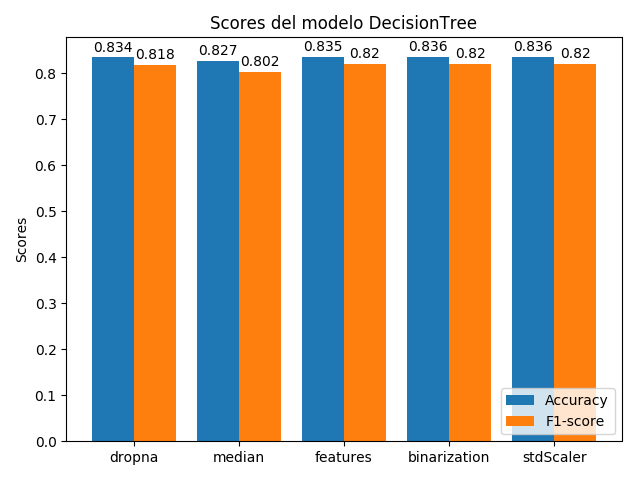
\includegraphics[width=90mm]{figures/visualizacion/decisionTree}
\end{figure}

La eficacia de Decision Tree no se vió afectada apenas por ninguno de
los procesamientos que planteamos. Trabaja con las variables por
separado, por lo que no le afecta el reescalado; trabaja bien con las
variables nominales, por lo que no se ve beneficiado de la
binarización de las mismas. Sí que observamos que este modelo
acostumbra a clasificar mejor las instancias negativas, ya que su
desempeño general (barra azul) está por encima de su F1-score (barra
naranja), que da mayor importancia a los ejemplos positivos.

\begin{figure}[H]
  \centering
  \label{fig:nb}
  \caption{Desempeño de Naive-Bayes para cada preprocesamiento}
  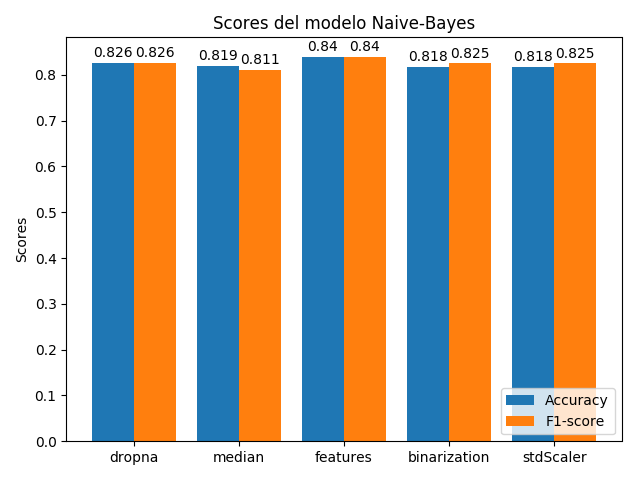
\includegraphics[width=90mm]{figures/visualizacion/gaussianNB}
\end{figure}

Sobre este modelo percibimos que funciona mejor tras la simplificación
del conjunto de características, pero empeora al introducir
características nuevas que no son independientes cuando binarizamos
las características nominales. Sobre algunos preprocesamientos ha
tenido similar desempeño al clasificar instancias positivas y
negativas (las barras azul y naranja están a la misma altura). Al
igual que el resto de modelos, al imputar los valores perdidos pierde
bastante efectividad sobre los ejemplos positivos (la barra naranja
está más abajo que la azul). Al introducir las características
dependientes en la binarización de variables nominales, decrece su
eficacia sobre todo para los ejemplos negativos (la barra naranja no
decrece tanto como la azul), y tampoco se ve afectado por el
reescalado de los datos.

\begin{figure}[H]
  \centering
  \caption{Desempeño de SVM para cada preprocesamiento}
  \label{fig:svm}
  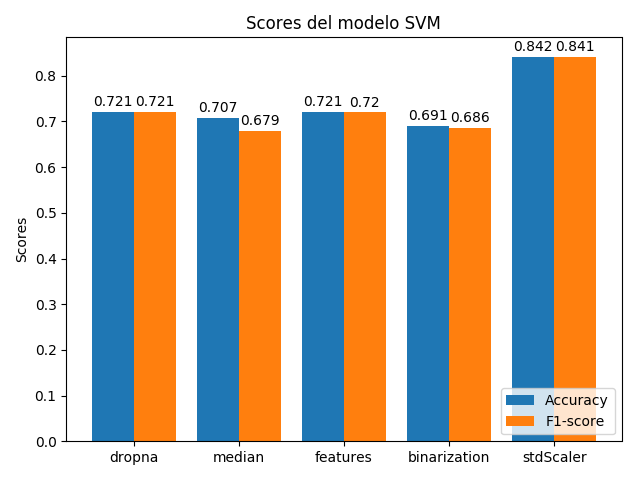
\includegraphics[width=100mm]{figures/visualizacion/svm}
\end{figure}

SVM presenta un desempeño bastante pobre hasta llegar al reescalado de
las variables, cuando se convierte en el modelo que más score
consigue. Se ve perjudicado por la binarización de características
nominales y, exceptuando lo que les ocurre a todos los algoritmos con
el segundo preprocesado (imputar valores perdidos), su desempeño es
similar en las características positivas y en las negativas (las
barras azul y naranja están muy igualadas).

\begin{figure}[H]
  \centering
  \caption{Desempeño de Random Forest para cada preprocesamiento}
  \label{fig:rf}
  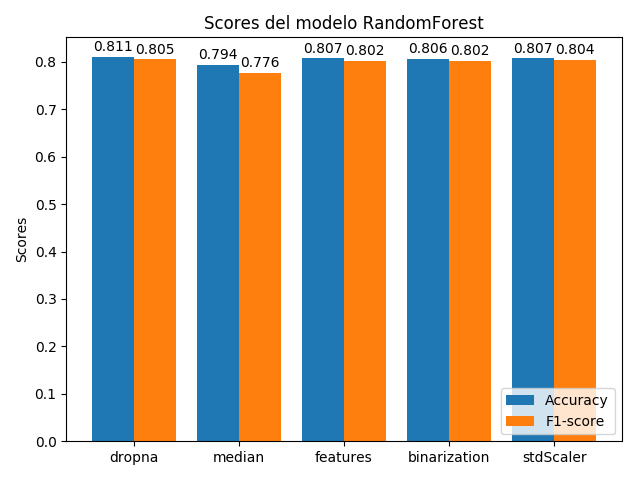
\includegraphics[width=100mm]{figures/visualizacion/randomForest}
\end{figure}

A Random Forest le ocurre lo mismo que a Decision Tree (Random Forest
es un modelo que promedia varios Decision Tree), aunque su desempeño
en general es peor. Hay un poco menos de diferencia entre las barras
azul y naranja, por lo que no empeora tanto al clasificar instancias
positivas.

\begin{figure}[H]
  \centering
  \caption{Desempeño de KNN para cada preprocesamiento}
  \label{fig:knn}
  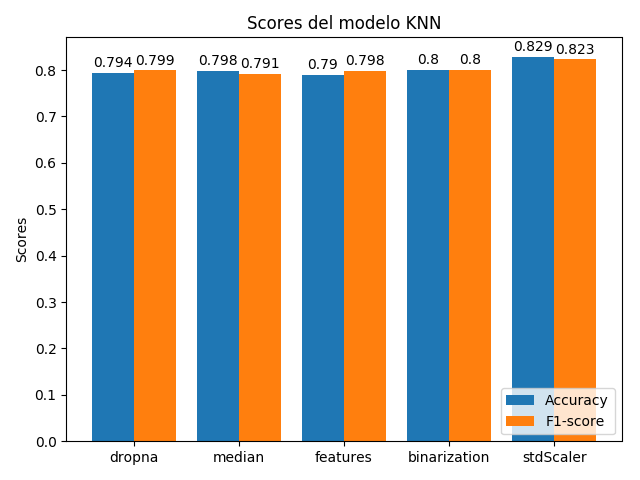
\includegraphics[width=100mm]{figures/visualizacion/knn}
\end{figure}

KNN se ve beneficiado por los dos últimos procesamientos, sobre todo
con el último, el reescalado de las variables. Presenta resultados
similares para todos los procesamientos, en comparación con los otros
modelos, empeora poco con la imputación de valores perdidos. Su
desempeño es similar para todos los preprocesamientos excepto para el
último, donde la mejora es notable.

\begin{figure}[H]
  \centering
  \caption{Desempeño de Neural Network para cada preprocesamiento}
  \label{fig:neuralNetwork}
  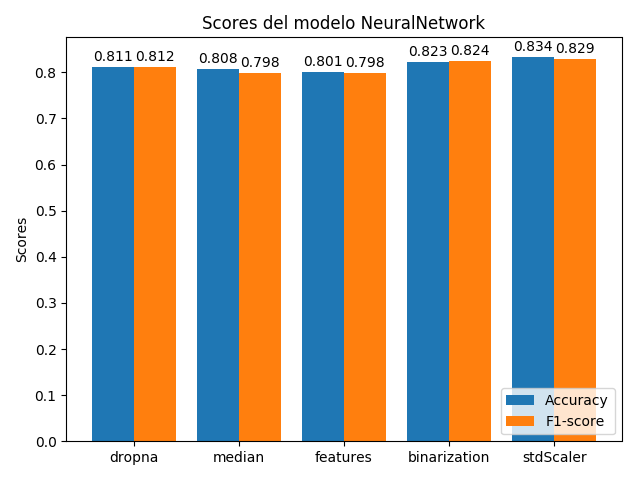
\includegraphics[width=100mm]{figures/visualizacion/neuralNetwork}
\end{figure}

Neural Network se ve perjudicado por la simplificación del conjunto de
características, probablemente porque es un modelo con una alta
complejidad y capacidad explicativa y sea capaz de aprovechas la poca
información que se pierde con esta simplificación. Los preprocesados
de binarización y estandarización le benefician en gran medida. En
general, su eficacia es similar en ejemplos positivos y negativos, las barras azul y naranja están prácticamente a la misma altura.

\section{Gráficas de la curva ROC}

Para cada preprocesamiento, compararemos los modelos representándolos
en el espacio ROC. Los estamos tratando como modelos discretos (sólo
atendemos a la clase que predigan, no la probabilidad que asignen de
pertenencia a cada clase), por lo que no vamos a dibujar sus curvas
ROC como es habitual verlas, con forma de codo. Esto podríamos hacerlo
con la función \texttt{roc\_curve} de \texttt{sklearn.metrics}, pero
tenemos que tener clara la interpretación continua que se hace del
modelo para interpretar las curvas. Por ejemplo un árbol de decisión
se puede interpretar como un modelo continuo de la siguiente manera:
si una instancia cae sobre una hoja con $p$ instancias de
entrenamiento de la clase maligno y $q$ de la clase benigno, puede
asignar una probabilidad de $\frac{p}{p+q}$ para la clase maligno y
una de $\frac{q}{p+q}$ para la clase benigno.

En su lugar, cada modelo aparecerá como un punto en el plano,
concretamente en el intervalo $[0,1]\times[0,1]$.

El análisis gráfico por gráfico sería muy repetitivo, por lo que nos
limitaremos a explicar cómo se interpretan estos gráficos. Lo haremos
sobre el primero de ellos. \vspace{-3mm}
\begin{figure}[H]
  \centering
  \caption{Algoritmos sobre el preprocesado 1 representados en el espacio ROC}
  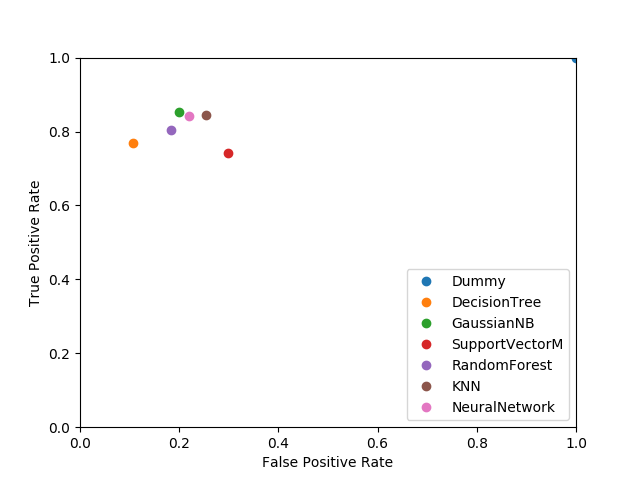
\includegraphics[width=120mm]{figures/visualizacion/roc1}
  \label{fig:roc1}
\end{figure}

En el eje horizontal se representa el FPR, la tasa de falsos positivos
(número de predicciones positivas incorrectas entre el número total de
ejemplos negativos). En el eje vertical se representa el TPR, la tasa
de verdaderos positivos (número de predicciones positivas correctas
entre el número total de ejemplos positivos).

Cuanto más a la izquierda esté un punto, menor será la FPR del modelo,
luego mejor clasificará ejemplos negativos. Cuanto más a arriba esté
un punto, mayor será la TPR del modelo, luego mejor clasificará
ejemplos positivos.

Si un modelo está situado arriba a la derecha de otro, significa que
predice mejor tanto los ejemplos positivos como los negativos, por lo
que podemos considerarlo mejor en cuanto a resultados, sin tener en
cuenta la simplicidad ni la facilidad de interpretación de los
modelos. De otra forma, dos modelos no son tan fácilmente comparables,
por lo que tendríamos que atender a sus diferencias de FPR y TPR, a la
importancia que le demos a cada una.

En este ejemplo concreto (Figura \ref{fig:roc1}), Naive-Bayes es mejor
que Neural Network, KNN y SVM. Obviamente Dummy supera a todos a la
hora de clasificar ejemplos positivos, pero es el peor clasificando
negativos. Naive-Bayes supera al árbol de decisión a la hora de
clasificar instancias positivas, pero es peor clasificando instancias
negativas. También apreciamos que SVM es el peor de todos sin contar
Dummy.

A continuación están las representaciones de los modelos en el espacio
ROC para el resto de preprocesamientos.

\begin{figure}[H]
  \centering
  \subfigure[Preprocesado 2: Imputación]{
    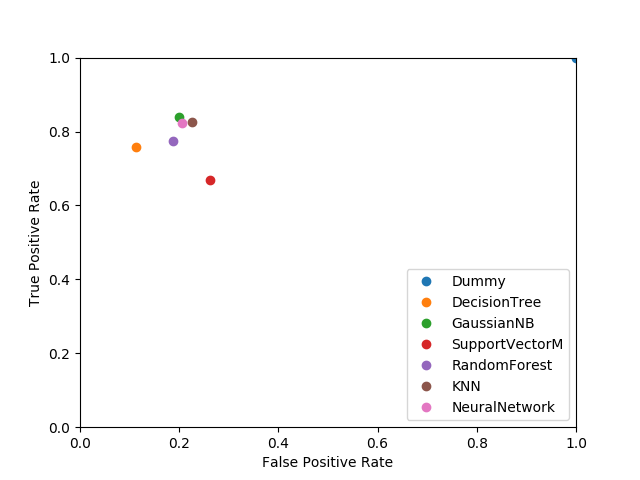
\includegraphics[width=85mm]{figures/visualizacion/roc2}
  }
  \subfigure[Preprocesado 3: Características]{
    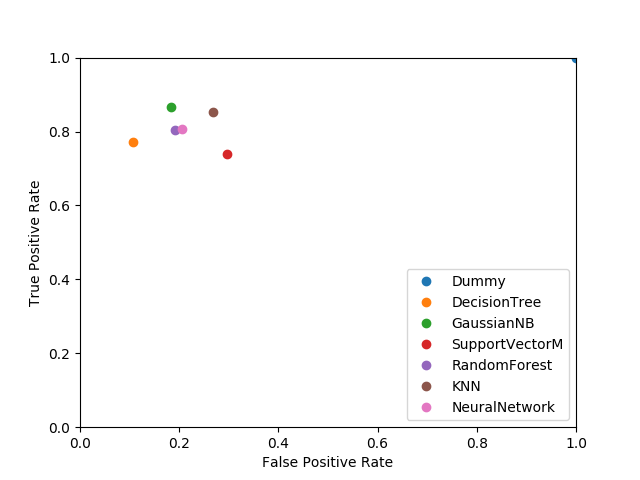
\includegraphics[width=85mm]{figures/visualizacion/roc3}
  }
  \subfigure[Preprocesado 4: Binarización]{
    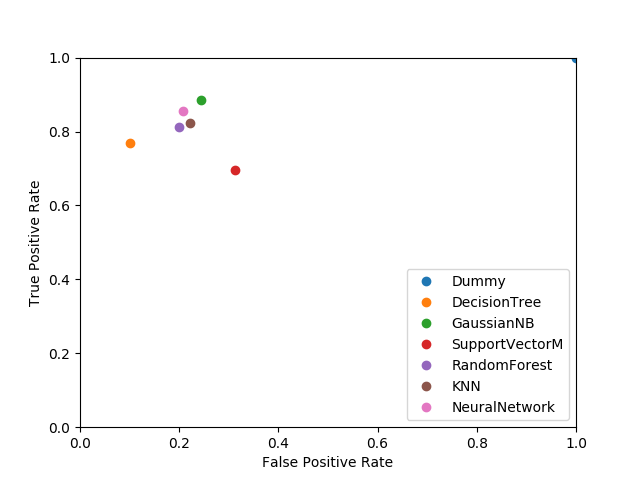
\includegraphics[width=85mm]{figures/visualizacion/roc4}
  }
  \subfigure[Preprocesado 5: Estandarización]{
    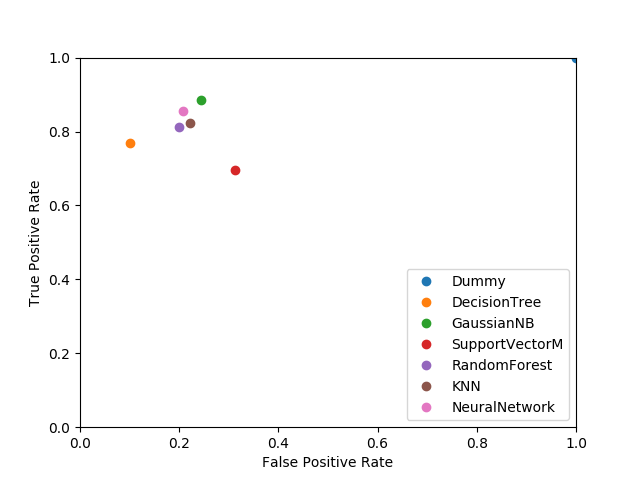
\includegraphics[width=85mm]{figures/visualizacion/roc4}
  }
  \caption{Algoritmos sobre cada preprocesado representados en el espacio ROC}
  \label{fig:roc2345}
\end{figure}

La métrica $AUC=\dfrac{1+TPR-FPR}{2}$ mide el área bajo la curva que
une el punto en el espacio con los puntos $(0,0)$ y $(1,1)$. En la
Figura \ref{fig:roc-auc} pueden observarse estas curvas para los
algoritmos con el preprocesamiento 1 (los de la Figura
\ref{fig:roc1}). Clarametente cuanto más arriba y a la izquierda esté
un punto, mayor será este área y por tanto la AUC del modelo. Esta
métrica es similar a Accuracy en el sentido que mide el desemepeño
general del modelo sin priorizar ninguna de las dos clases
(positiva/negativa), con la diferencia de que equilibra la importancia
de las clases sin importar lo balanceadas que estén, por tanto es
recomendable utilizar AUC cuando tenemos clases desbalanceadas y
queremos evitar que se ignore/desprecie la clase minoritaria.

En la Tabla \ref{tab:auc}, recogemos los distintos valores de este
área para los modelos sobre el preprocesado 1 (Figura \ref{fig:roc1} o
Figura \ref{fig:roc-auc}) y también sobre el resto de preprocesamientos (Figura \ref{fig:roc2345}).

\begin{figure}[H]
  \centering
  \caption{Curvas ROC de los algoritmos sobre el preprocesado 1}
  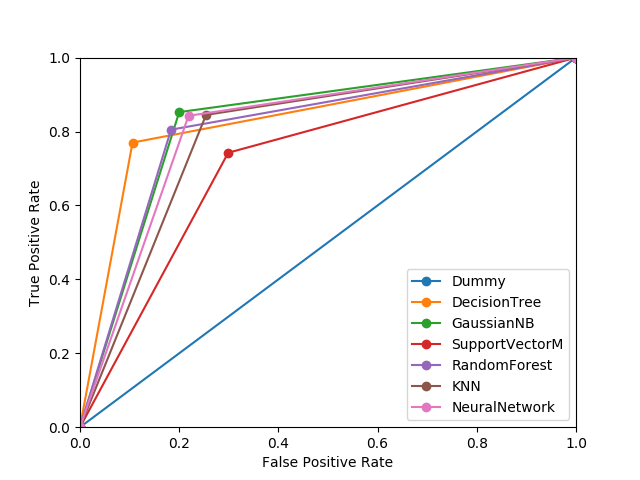
\includegraphics[width=120mm]{figures/visualizacion/roc-auc}
  \label{fig:roc-auc}
\end{figure}

\begin{table}[H]
  \centering
  \begin{tabular}{|l|ccccccc|} \hline
     & Dummy & DecisionTree & GaussianNB & SupportVectorM & RandomForest & KNN & NeuralNetwork \\ \hline
Preprocesado 0 & 0.5 & 0.832 & 0.8262 & 0.7219 & 0.8108 & 0.7954 & 0.8118 \\ \hline
Preprocesado 1 & 0.5 & 0.8224 & 0.8204 & 0.704 & 0.7925 & 0.8001 & 0.8086 \\ \hline
Preprocesado 2 & 0.5 & 0.8333 & 0.8408 & 0.7218 & 0.8072 & 0.7922 & 0.8014 \\ \hline
Preprocesado 3 & 0.5 & 0.8344 & 0.8202 & 0.691 & 0.8062 & 0.8006 & 0.824 \\ \hline
Preprocesado 4 & 0.5 & 0.8344 & 0.8202 & 0.843 & 0.8076 & 0.8288 & 0.8339 \\ \hline
  \end{tabular}
  \caption{AUC de cada modelo y procesamiento}
  \label{tab:auc}
\end{table}

\newpage

\section{Análisis de atributos}

Para cada atributo, representamos para cada posible valor el número de
instancias positivas (en azul) y negativas (en naranja). Utilizamos un
gráfico de barras apiladas, con el número de instancias malignas
abajo. En este tipo de gráficos será fácil saber cuantas instancias
malignas tienen determinado valor de una variable, y también cuantas
instancias totales. Para ver el número de instancias benignas habrá
que tener en cuenta donde empieza la barra.

\begin{figure}[H]
  \centering
  \caption{Distribución de ejemplos de cada clase para los distintos valores de BI-RADS}
  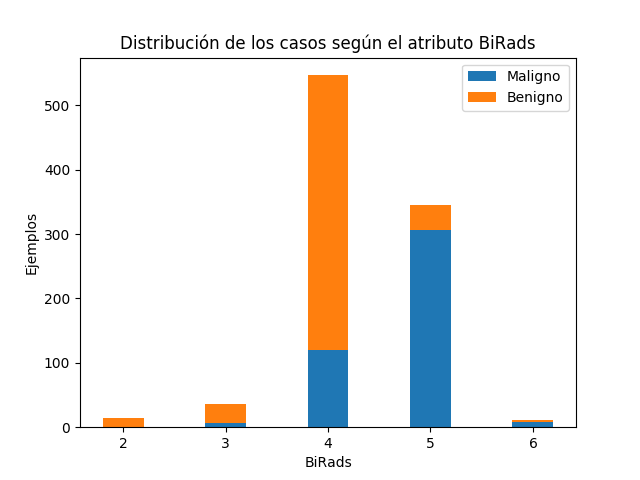
\includegraphics[width=140mm]{figures/visualizacion/birads}
  \label{fig:birads}
\end{figure}

La mayoría de instancias tienen los valores 4 y 5. Al aumentar el
valor de la variable, aumenta considerablemente la proporción de
ejemplos malignos con ese valor. Por tanto, vemos que esta variable
está altamente relacionada con la severidad del tumor.

\begin{figure}[H]
  \centering
  \caption{Distribución de ejemplos de cada clase para los distintos valores de Age}
  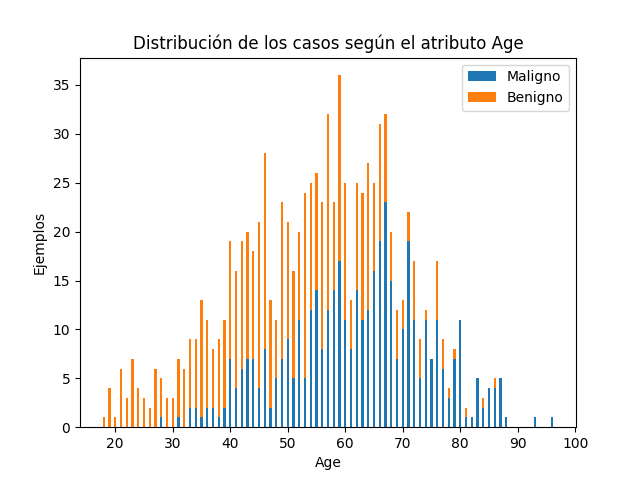
\includegraphics[width=120mm]{figures/visualizacion/age}
  \label{fig:age}
\end{figure}

Al haber tantos valores es lógico que halla impurezas, pero al igual
que antes, observamos un aumento en la proporción de ejemplos malignos
para valores altos de la variable. Por lo que también concluimos que
la edad está bastante relacionada con la severidad.

\begin{figure}[H]
  \centering
  \caption{Distribución de ejemplos de cada clase para los distintos valores de Density}
  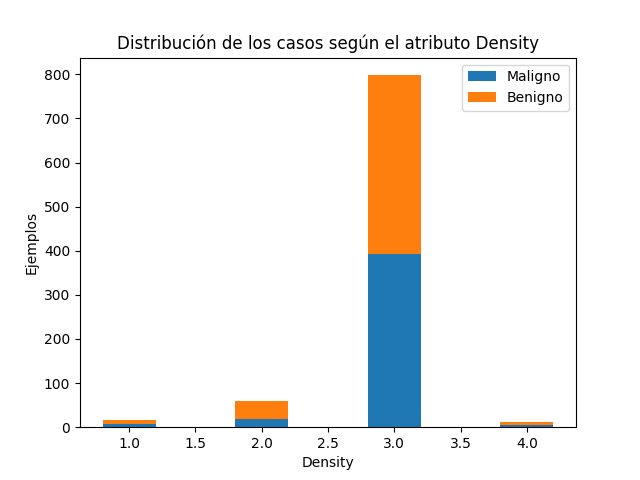
\includegraphics[width=120mm]{figures/visualizacion/density}
  \label{fig:density}
\end{figure}

Observamos que la mayoría de las instancias presentan el valor 3 de
esta variable. Además, para cada valor el número de instancias
positivas y negativas que lo presentan es prácticamente el mismo. Por
tanto, no parece que esta variable influya en la severidad del tumor.

\begin{figure}[H]
  \centering
  \caption{Distribución de ejemplos de cada clase para los distintos valores de Margin}
  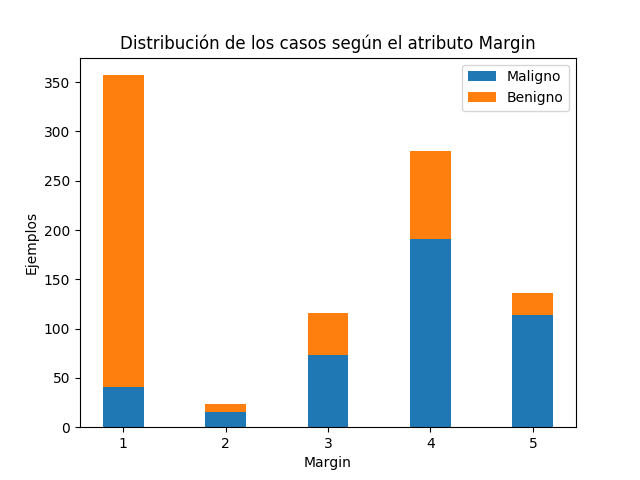
\includegraphics[width=115mm]{figures/visualizacion/margin}
  \label{fig:margin}
\end{figure}

La mayoría de las instancias que presentan el valor 1 corresponden a
tumores benignos y la mayortía de las que presentan el valor 5, a
malignos. Para el resto de valores (2, 3 y 4), la proporción de
instancias malignas es mayor que la de benignas. Concluimos que este
atributo sí puede aportarnos información sobre la severidad del tumor.

\begin{figure}[H]
  \centering
  \caption{Distribución de ejemplos de cada clase para los distintos valores de Shape}
  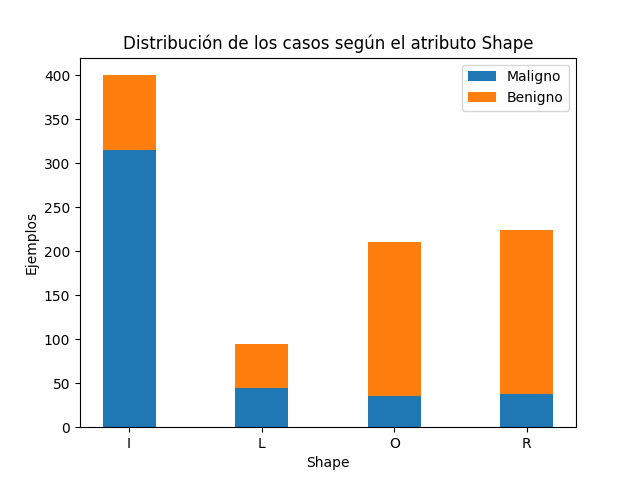
\includegraphics[width=115mm]{figures/visualizacion/shape}
  \label{fig:shape}
\end{figure}

La mayoría de instancias que presentan el valor I de esta variable,
corresponden a tumores malignos. La mayoría de las instancias que
presentan los valores O o R de esta variable, corresponden a
benignos. Mientras que hay aproximadamente las mismas instancias
benignas que malignas entre las que tienen valor L. Por tanto, esta
variable también está relacionada con la severidad.

\begin{center}
\vspace*{8cm}
\part{\textbf{Segmentación}}
\end{center}

\setcounter{section}{0}
\renewcommand*{\theHsection}{\theHpart.\the\value{section}}

\section{Introducción}

En esta práctica emplearemos técnicas de aprendizaje no supervisado,
como es el clustering, para realizar un análisis relacional mediante
segmentación.

Nuestro dataset consta de todos los accidentes ocurridos en España
durante el año 2013. Los datos están publicados por la
\href{https://sedeapl.dgt.gob.es/WEB_IEST_CONSULTA/subcategoria.faces}{DGT}. Disponemos
de datos de 89519 accidentes, y 32 variables que miden circunstancias
en las que ocurre cada accidente (día, hora, visibilidad, superficie
de la calzada, factores atmosféricos, zona \ldots), el tipo (alcance,
choque frontal, choque lateral, atropello a peatón o animal, colisión
con obstáculo \ldots) y la gravedad (número de heridos leves y graves y
número de muertos).

Los algoritmos de clustering que utilizaremos son:
\begin{itemize}
\item \href{https://en.wikipedia.org/wiki/K-means_clustering}{\textbf{K-means:}} Un algoritmo iterativo basado en
  particionamiento. Es relativamente eficiente ($O(tkn)$ donde $n$ es
  el número de datos, $k$ el de clusters y $t$ el de iteraciones) y
  suele alcanzar óptimos locales bastante buenos. Por otra parte, sólo
  trabaja bien cuando los datos son numéricos, necesita prefijar el
  número de clusters, sólo encuentra clusters esféricos y no lidia
  bien con datos ruidosos y outliers.

\item
  \href{https://en.wikipedia.org/wiki/DBSCAN}{\textbf{DBSCAN:}}
  También basado en particionamiento. No necesita a priori el número
  de clusters, en su lugar requiere el radio máximo de cada cluster y
  el tamaño mínimo de los mismos. También es capaz de encontrar
  clusters con distintas formas y es robusto a datos ruidosos y
  outliers.

\item \href{https://en.wikipedia.org/wiki/Ward%27s_method}
    {\textbf{Ward:}} Es un método aglomerativo, es decir, parte de un
    cluster para cada elemento y fusiona los clusters que generen en
    el agrupamiento con mínima varianza. Necesita el número de cluster
    o una distancia límite a partir de la cual no fusiona dos
    clusters.
\end{itemize}

Para estimar los hiperparámetros de los algoritmos atenderemos a dos
métricas para interpretar la bondad de un agrupamiento:

\begin{itemize}
\item \href{https://en.wikipedia.org/wiki/Silhouette_%28clustering%29}
    {\textbf{Coeficiente Silhouette:}} Compara la similitud de de los
    objetos de un mismo cluster (cohesión) con los de otros clusters
    (separación). Para cada elemento $i$, se calcula $a(i)$ como la
    distancia media entre $i$ y el resto de elementos del cluster,
    mientras que que $b(i)$ representa el mínimo de las distancias
    entre $i$ y cada cluster distinto del suyo (la distancia de $i$ a
    un cluster se calcula como la media de las distancias de $i$ a
    cada elemento del cluster). Tomando
    \[s(i)=\frac{b(i)-a(i)}{\max{a(i),b(i)}}\] se tiene
    $s(i)\in[-1,1]$. Si $s(i)$ es negativo \big($b(i)<a(i)$\big),
    claramente el elemento $i$ pertenece al cluster equivocado (está
    más cerca de un cluster distinto al suyo); si $s(i)$ está cerca de
    1, significa que $i$ está mucho más cerca de los elementos de su
    cluster que del resto de clusters. El coeficiente silhoutte se
    calcula como la media de los $s(i)$ para todos los ejemplos
    $i$. Usualmente se encuentra entre 0 y 1.

  \item
    \href{https://www.tandfonline.com/doi/pdf/10.1080/03610927408827101?needAccess=true}{\textbf{Razón
        de Calinski-Harabasz:}} Razón entre la dispersión
    intra-clusters (dentro de cada cluster) cantidad que y la
    dispersión inter-clusters (entre clusters). Su cálculo es más
    complejo que el anterior y su valor no está entre 0 y 1, en
    nuestro caso toma valores del orden de miles.
  \end{itemize}

  Otro factor muy importante a tener en cuanta será el número de
  clusters generados, ya un elevado número de clusters dificulta las
  tareas de interpretación y análisis de los resultados. El hecho de
  generar un número excesivo de clusters con el fin de maximizar las
  métricas al precio de dificultar el análisis y la interpretabilidad
  sería el equivalente a lo que en aprendizaje supervisado conocíamos
  como sobreajuste, podemos llamarle también de ese
  modo. Representaremos los scores frente al número de cluster en
  gráficas y elegiremos los hiperparámetros por un criterio similar al
  \href{https://en.wikipedia.org/wiki/Elbow_method_%28clustering%29}
    {método del codo}, a partir de la gráfica intentaremos determinar
    cuando la ganancia de score deja de compensar el aumento en el
    número de clusters.

  Debido al elevado número de datos, los algoritmos de clustering (que
  suelen presentar un elevado orden de complejidad) podrían tardar un
  tiempo excesivo en ejecutarse, por lo que realizaremos dos casos de
  estudio en cada uno de los cuales seleccionaremos un subconjunto de
  las instancias. Para cada caso de estudio, restringiremos el número
  de datos fijando los valores de una o más variables de carácter
  circunstancial o de tipo, y realizaremos el agrupamiento basándonos
  en las variables que miden la gravedad de los accidentes, pues son
  numéricas y nos evitan problemas como la dificultad de K-means para
  trabajar con variables nominales.

  Existe una amplia variedad de casos de estudio con sentido e interés
  que podríamos analizar: accidentes bajo condiciones climatológicas
  adversas frente a buen tiempo, en zonas urbanas frente a
  interurbanas, atropellos, colisiones, etc. Nosotros analizaremos los
  accidentes en condiciones óptimas para la conducción y los
  accidentes que ocurren a altas horas de la madrugada. En cada caso
  de estudio, realizaremos segmentación con dos algoritmos, K-means y
  uno de los otros.

  Es importante normalizar los datos (reescalarlos por columnas para
  que estén en el intervalo $[0,1]$ antes de realizar la segmentación
  para que los algoritmos funcionen correctamente. De lo contrario,
  algunas dimensiones cobrarían más importancia que otras. Para ello,
  utilizamos
  \href{https://scikit-learn.org/stable/modules/generated/sklearn.preprocessing.MinMaxScaler.html}{\texttt{MinMaxScaler}}
  de \textit{sklearn}.

  Para ciertas tareas como el cálulo de las métricas y la
  visualización de los centroides y las distribuciones por pares de
  atributos en los clusters, utilizamos las funciones que se nos
  proporcionan en el fichero \texttt{pract2\_utils.py}, que
  internamente utiliza \textit{skleran} para las métricas y
  \textit{seaborn} para las visualizaciones. Hemos relizado pequeñas
  modificaciones en este fichero: la posibilidad de introducir los
  centroides ya desnormalizados para su visualización y cambios en las
  paletas de colores para hacer las visualizaciones más fácilmente
  interpretables.
  
  \section{Caso de estudio 1: Análisis de los accidentes en
    condiciones óptimas para la conducción}

  Para este primer caso de estudio, seleccionamos los accidentes que
  ocurren en condiciones óptimas para la conducción. Estos accidentes
  pueden ocurrir bien por factor vehículo o bien por factor humano, ya
  que eliminaremos el factor vía seleccionando ejemplos de accidentes
  que ocurren en calzadas secas y limpias. No disponemos de datos
  relativos al factor vehículo, pero dentro del factor humano,
  eliminaremos también las condiciones que favorecen los errores
  humanos como la falta de luminosidad, visibilidad o la circulación
  densa. Teniendo en cuenta que el factor vehículo es causa de un
  porcentaje relativamente bajo de accidentes (menos del 10\%),
  principalmente tenemos accidentes debidos al factor humano que han
  ocurrido en condiciones óptimas para la conducción: buen tiempo,
  buena visibilidad, calzada limpia y seca, tráfico fluido, etc. Es
  decir, accidentes debidos a factor humano que se podrían haber
  evitado. Aquí radica el interés de este caso de estudio.

En concreto, estos son los valores que fijamos para las variables:

\begin{verbatim}
LUMINOSIDAD=='NOCHE: ILUMINACIÓN SUFICIENTE' | LUMINOSIDAD=='PLENO DÍA'
DENSIDAD_CIRCULACION=='FLUIDA'
DIASEMANA==6
OTRA_CIRCUNSTANCIA=='NINGUNA'
FACTORES_ATMOSFERICOS=='BUEN TIEMPO'
MEDIDAS_ESPECIALES=='NINGUNA MEDIDA'
SUPERFICIE_CALZADA=='SECA Y LIMPIA'
VISIBILIDAD_RESTRINGIDA=='SIN RESTRICCIÓN'
\end{verbatim}

Con \texttt{OTRA\_CIRCUNSTANCIA=='NINGUNA'} descartamos accidentes
ocurridos con obras, inundaciones, baches, badenes, cambios de
rasante, estrechamientos, pasos a nivel y demás circunstancias que
podrían dificultar la conducción. Con
\texttt{MEDIDAS\_ESPECIALES=='NINGUNA MEDIDA'} descartamos accidentes
ocurridos en carriles reversibles o con habilitación del arcén, que
podríamos considerar fuera de la conducción ``normal''.

Además, para quedarnos con menos datos nos restringimos a los
accidentes ocurridos en sábado con \texttt{DIASEMANA==6}. Los días del
lunes al jueves son más propensos a presentar accidentes con una sola
víctima (como apreciamos en la Figura \ref{fig:diasemana}), esto ocurre
porque va mucha más gente a trabajar, mientras que en fin de semana es
más usual que viajen varias personas en el coche. Así que elegimos
este día para obtener un mayor número de accidentes con múltiples
víctimas. El hecho de que viajen más personas en el coche a parte del
conductor, por una parte puede aumentar la responsabilidad y por otra
puede aumentar las distracciones o crear una falsa sensación de
confianza. Esto hace los accidentes ocurridos en fin de semana más
interesantes, en mi opinión. Motivo por el cuál elegimos un día del
fin de semana.

\begin{figure}[H]
  \centering
  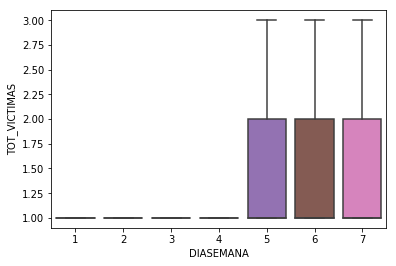
\includegraphics[width=140mm]{figures/accidentes/diasemana}
  \caption{De lunes a jueves la mayoría de accidentes ocasionan una
    sola víctima (considera los accidentes con más víctimas como
    outliers). En fin de semana hay más accidentes con múltiples
    víctimas.}
  \label{fig:diasemana}
\end{figure}
\vspace{-5mm}
Fijando estos valores, nos quedamos con 4143 instancias, por lo que
nuestros algoritmos se ejecutarán bastante rápido.

Anticipando problemas posteriores, debemos eliminar los outliers para
poder visualizar la segmentación correctamente. Utilizando
\texttt{Counter} observamos que hay un accidente con 52 víctimas, esto
distorsiona las escalas de los ejes en las gráficas de víctimas y
heridos, lo que dificulta su interpretación.

Por tanto, eliminamos los outliers con el siguiente código, que
colapsa los valores por encima del máximo de la whisker box, que
admite hasta la media más 3 por la desviación típica
($\mu+3\cdot\sigma$), en dicho máximo.

\begin{verbatim}
# Eliminar outliers, ya que distorsionan las gráficas
for a in atributos:
    if a in {'TOT_MUERTOS','TOT_HERIDOS_GRAVES'}:
        continue
    d=data[a][abs(zscore(data[a]))<3]
    data[a][zscore(data[a])<-3]=d.min()
    data[a][zscore(data[a])>3]=d.max()
\end{verbatim}

La gran mayoría de accidentes no presenta muertos ni heridos graves,
lo que provoca que los muertos y heridos graves se consideren
outliers, por eso los dejamos tal y como están. En la siguiente
gráfica podemos comparar las distribuciones de las variables, se
elminan la mayoría de outliers y se regula la escala de los ejes,
salvo en los dos atributos que no hemos modificado.

Adelantando acontecimientos, esta limpieza de los datos presenta
inconvenientes que discutimos en la Sección \ref{sec:outliers}.

\begin{figure}[H]
  \centering
  \subfigure[Antes de eliminar outliers.]{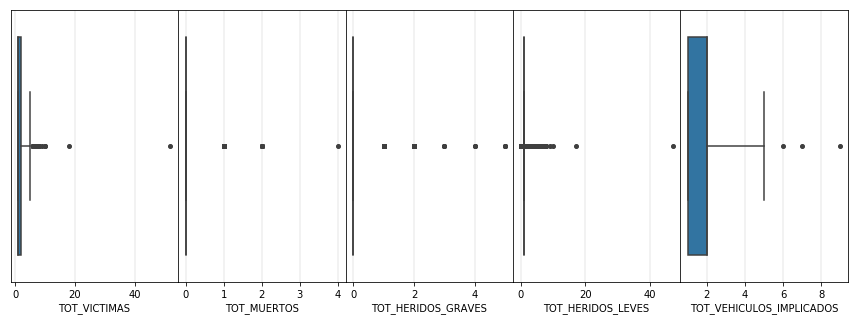
\includegraphics[width=160mm]{figures/accidentes/outliers1}}
  \subfigure[Tras eliminar outliers.]{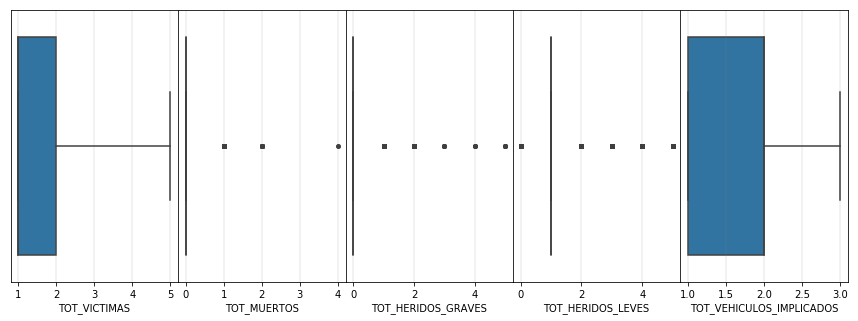
\includegraphics[width=160mm]{figures/accidentes/outliers2}}
  \caption{Distribución de los valores de cada variable.}
  \label{fig:distrib1-outliers}
\end{figure}

\subsection{Algoritmos de clustering y resultados} \label{sec:alg1}

El primer algoritmo que probaremos para abordar este problema es
\textbf{K-means}, utilizaremos la
\href{https://scikit-learn.org/stable/modules/generated/sklearn.cluster.KMeans.html}{implementación}
del módulo de clusters de \textit{sklearn}. En primer lugar debemos
escoger un valor de $K$ adecuado, para ello nos basamos en las
métricas Silhouette y Calinski(-Harabasz). Probando diferentes valores
de $K$, obtenemos la siguiente tabla:

\begin{table}[H]
  \centering
\begin{tabular}{|c|cc|}
  \hline
  ~\hspace{2mm}K\hspace{2mm}~ & ~\hspace{2mm}Calinski\hspace{2mm}~ & ~\hspace{2mm}Silhouette\hspace{2mm}~ \\ \hline
2 & 3042.33 & 0.5541 \\ \hline
3 & 4703.28 & 0.6437 \\ \hline
4 & 4136.87 & 0.6577 \\ \hline
5 & 4038.97 & 0.6892 \\ \hline
6 & 3853.22 & 0.7027 \\ \hline
7 & 4151.42 & 0.7369 \\ \hline
8 & 4226.28 & 0.7867 \\ \hline
9 & 4805.5 & 0.8417 \\ \hline
\end{tabular}
\caption{Scores de K-means para distinto número de clusters.}
\label{tab:k-means1}
\end{table}

Nos ayudamos de representaciones gráficas para elegir un valor de $K$
adecuado. Buscamos un valor bajo para $K$ y valores altos para las
métricas.

\begin{figure}[H]
  \centering
  \subfigure[Razón de Calinski-Harabasz]{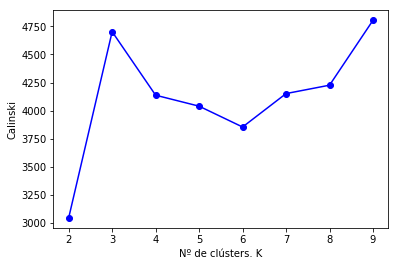
\includegraphics[width=87mm]{figures/accidentes/k-means1cal}}
  \subfigure[Coeficiente Silhouette]{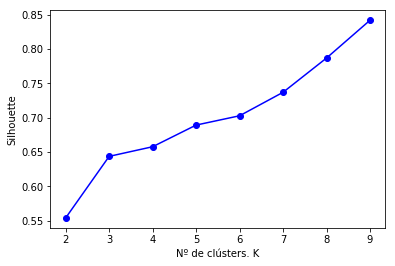
\includegraphics[width=87mm]{figures/accidentes/k-means1sil}}
  \caption{Representaciones de los scores de K-means para distinto número de clusters.}
  \label{fig:k-means1-scores}
\end{figure}

La gráfica de Calinski claramente sugiere tomar $K=3$, ya que presenta
un máximo local bastante alto, sólo superado por $K=9$ y no por
mucho. En cambio, la gráfica de Silhouette no experimenta una ganancia
tan abrupta para este valor, pero la ganancia es aun más suave para
valores posteriores, por lo que de no tomar $K=3$, sugeriría tomar
$K=8$ o $K=9$. Esto complica bastante la posterior interpretación de
la segmentación, por lo que nos decantamos por $K=3$.

El siguiente código realiza el agrupamiento y obtiene las etiquetas
(el cluster al que pertenece cada ejemplo) y los centroides de cada
cluster.

\begin{verbatim}
K=3
results = KMeans(n_clusters=K, random_state=0).fit(data_norm)
labels=results.labels_
centroids=results.cluster_centers_
\end{verbatim}

Con \texttt{Counter}, consultamos el tamaño (número de elementos) de
cada cluster. Observamos que el cluster 0 es bastante más pequeño que
los otro dos.
\begin{verbatim}
Counter(labels)
> Counter({0: 419, 1: 1673, 2: 2051})
\end{verbatim}

Dejaremos la visualización de los centroides y de las distribuciones
de los clusters para la interpretación, en la Sección
\ref{sec:interpretacion1}. Relizaremos ahora el agrupamiento con el
algoritmo \textbf{Ward}, un método acumulativo. La implementación que
usamos es la de
\href{https://scikit-learn.org/stable/modules/generated/sklearn.cluster.AgglomerativeClustering.html}{clustering
  aglomerativo} de \textit{sklearn}, indicando Ward (mínima varianza)
como criterio para fusionar clusters (parámetro \texttt{linkage}).

Para seleccionar un número adecuado de clusters, realizamos un
experimento análogo al de la Tabla \ref{tab:k-means1}. Obteniendo:

\begin{table}[H]
  \centering
\begin{tabular}{|c|cc|}
  \hline
  ~\hspace{2mm}K\hspace{2mm}~ & ~\hspace{2mm}Calinski\hspace{2mm}~ & ~\hspace{2mm}Silhouette\hspace{2mm}~ \\ \hline
2 & 3038.94 & 0.5539 \\ \hline
3 & 3263.5 & 0.6002 \\ \hline
4 & 3211.22 & 0.6236 \\ \hline
5 & 3504.66 & 0.6674 \\ \hline
6 & 3925.91 & 0.715 \\ \hline
7 & 3951.38 & 0.7541 \\ \hline
8 & 4090.58 & 0.7905 \\ \hline
9 & 4256.87 & 0.8254 \\ \hline\end{tabular}
\caption{Scores de Ward para distinto número de clusters.}
\label{tab:ward1}
\end{table}

\begin{figure}[H]
  \centering
  \subfigure[Razón de Calinski-Harabasz]{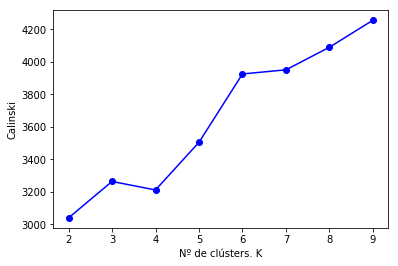
\includegraphics[width=87mm]{figures/accidentes/ward1cal}}
  \subfigure[Coeficiente Silhouette]{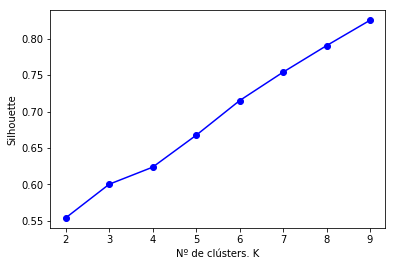
\includegraphics[width=87mm]{figures/accidentes/ward1sil}}
  \caption{Representaciones de los scores de Ward para distinto número de clusters.}
  \label{fig:ward1-scores}
\end{figure}

La métrica de Calinski sugiere los valores $K=3$ y $K=6$, mientras que
Silhouette crece prácticamente de forma lineal. Tomaremos $K=6$, ya
que la ganancia en la métrica de Calinski es significativa y así
tendremos la oportunidad de analizar un agrupamiento con un número de
clusters algo mayor.

El siguiente código realiza el agrupamiento y obtiene las etiquetas
(el cluster al que pertenece cada ejemplo).

\begin{verbatim}
K=6
results = AgglomerativeClustering(distance_threshold=None, n_clusters=K).fit(data_norm)
labels=results.labels_
\end{verbatim}

Este algoritmo no devuelve los centroides, para calcularlos agrupamos
los datos por etiqueta y hacemos la media de cada atributo.

\begin{verbatim}
dataC=data.copy()
dataC['cluster']=labels
centroids = dataC.groupby('cluster').mean()
\end{verbatim}

Vemos que hay diferentes tamaños de cluster.

\begin{verbatim}
Counter(labels)
> Counter({0: 1493, 1: 549, 2: 1535, 3: 140, 4: 264, 5: 162})
\end{verbatim}

\subsection{Interpretación de la
  segmentación} \label{sec:interpretacion1}

Comenzaremos por el agrupamiento generado por el algoritmo
K-means. Visualizamos los centroides con la función
\texttt{visualize\_centroids} del fichero \texttt{pract2\_utils.py}.
Visualizamos también cómo se distribuyen los valores de las variables
en cada cluster.

Visualizar los centroides nos da una idea del tipo de accidentes en
cada cluster, pero visualizar la distribución de las variables en un
diagrama de cajas y bigotes nos proporciona más información. Porque
podemos saber cómo de cerca están los elementos del cluster de ese
centroide. Si vemos una sola línea, significa que la mayoría de
elementos del cluster tienen ese valor, los suficientes para
considerar el resto como outliers.

\begin{figure}[H]
  \centering
  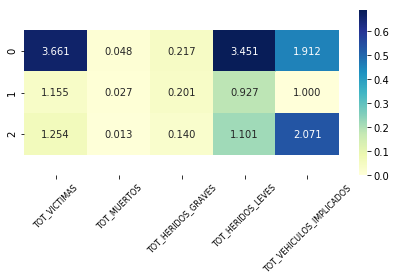
\includegraphics[width=120mm]{figures/accidentes/k-means1centroids}
  \caption{Centroides de los clusters generados por K-means.}
  \label{fig:k-means1centroids}
\end{figure}

\begin{figure}[H]
  \centering
  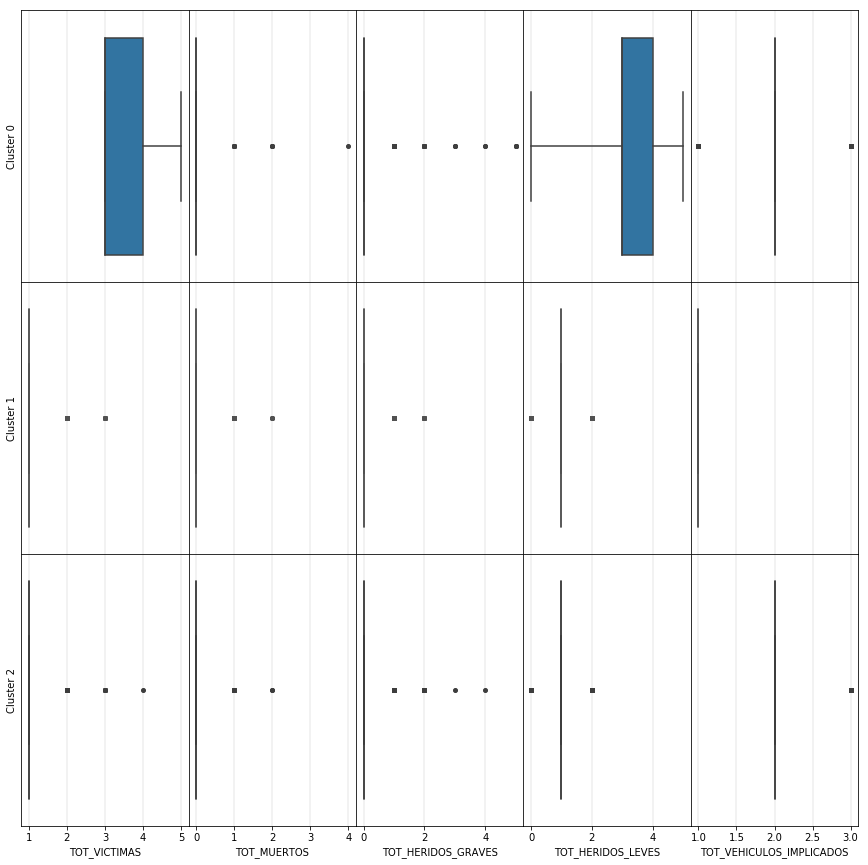
\includegraphics[width=130mm]{figures/accidentes/k-means1distribution}
  \caption{Distribución de las variables en los clusters generados por
    K-means.}
  \label{fig:k-means1distribution}
\end{figure}


Tenemos el cluster 0, que agrupa los accidentes con 3 o más víctimas,
la mayoría de las cuales son heridos leves. Generalmente son
accidentes con dos vehículos implicados, aunque en la Figura
\ref{fig:k-means1centroids} apreciamos que debe haber algunos
accidentes con un sólo vehículo implicado (la media es ligeramente
menor a 2), pero la Figura \ref{fig:k-means1distribution} vemos que
estos casos constituyen un porcentaje tan bajo que los considera
outliers. Los elementos de este cluster probablemente representen en
su mayoría choques frontales/laterales de vehículos, que suelen ser
los que más víctimas ocasionan.

En el cluster 1, tenemos accidentes con generalmente una vícitma (que
acostumbra a ser leve) y un vehículo implicado. Podrían tratarse, por
ejemplo, de choques de un solo vehículo con un obstáculo, generalmente
con un sólo conductor y leves. En la Figura
\ref{fig:k-means1distribution} apreciamos que en algunas ocasiones
(outliers) hay más heridos o de mayor gravedad, pero en el caso de los
vehículos implicados únicamente hay accidentes con un vehículo
implicado.

Por último, el cluster 2 agrupa accidentes con dos vehículos
implicados pero con bajo número de víctimas y generalmente
leves. Pueden tratarse en su mayoría de colisiones por alcance, que
acostumbran a ser más leves que el resto de colisiones. Aunque la
Figura \ref{fig:k-means1centroids} nos dice que deben existir en este
cluster accidentes don más de dos vehículos implicados (la media es
ligeramente mayor que 2), en la Figura \ref{fig:k-means1distribution}
observamos que son una minoría (los considera outliers).

Atendiendo al tamaño de los clusters, observamos que los accidentes
leves con dos vehículos implicados son los más comunes (cluster 2,
$\sim$49.5\%), le siguen los accidentes leves con un vehículo
implicado (cluster 1, $\sim$40.4\%). Y por último, los accidentes con
un mayor número de víctimas y generalmente dos vehículos implicados
(cluster 0, $\sim$10.1\%). Así nos hacemos una idea de la frecuencia
de cada tipo de accidente en las condiciones descritas en el caso de
estudio.

Debemos resaltar que la proporción de muertos y heridos graves es
demasiado baja como para que se consideren a la hora de agrupar por
los datos, en la Figura \ref{fig:k-means1distribution} observamos que
los valores distintos de 0 para estas dos variables los considera
outliers. Nos surge aquí la siguiente duda que tendremos la
oportunidad de responder más adelante: ¿Al aumentar el número de
clusters tendrá en cuenta los valores de estas variables para agrupar?
En caso afirmativo, ¿a partir de qué número de clusters? ¿merecerá la
pena aumentar el número de cluster o esto provocará también que se
``fuerce la separación'' de clusters que tiene perfecto sentido
fusionar? Lo que sería sobreajuste.

Los 4143 accidentes acumulan 92 muertos y 714 heridos graves.

Podemos también visualizar los cluster en un \textit{pairplot} para
observar la relación entre las variables dos a dos, así como la
distribución de los valores de las variables en cada cluster.

\begin{figure}[H]
  \centering
  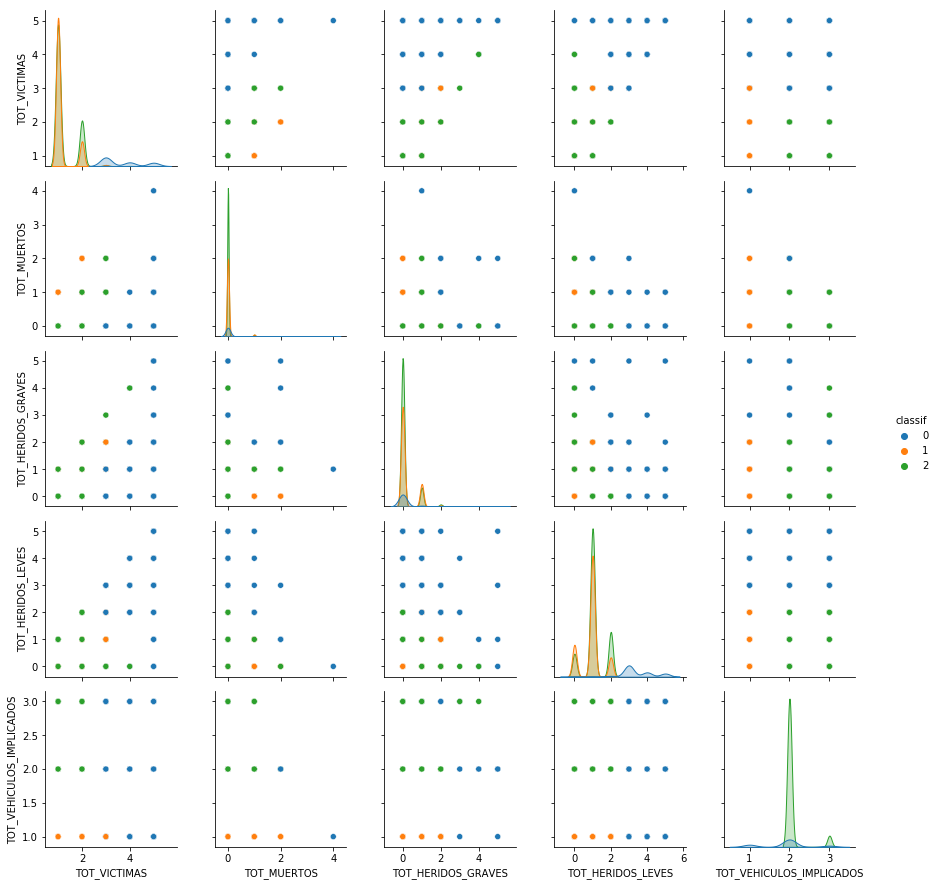
\includegraphics[width=180mm]{figures/accidentes/k-means1pair}
  \caption{Distribución de las variables en los clusters generados por
    K-means, por pares.}
  \label{fig:k-means1pair}
\end{figure}

En las diagonales, observamos las distribuciones para cada cluster de
los valores del atributo correspondiente. Por ejemplo en los heridos
leves y en el núemero de víctimas observamos que el cluster 0 llega a
tomar valores más altos (la distribución está más a la derecha),
mientras que en los otros dos clusters hay poca diferencia, el cluster
2 (verde) toma el valor 2 con ligeramente más frecuencia. Si
observamos los muertos, concluimos que esta variable no nos ayuda a
diferenciar los clusters, porque todos tienen su distribución
prácticamente degenerada en 0. Si observamos en la diagonal los
vehículos implicados, vemos que no aparece el cluster 1 por tomar
todos sus elementos el valor 1 para esta variable, lo que hace que la
``línea'' tenga grosor 0. Esto nos lo advierte un warning (Dataset has
0 variance; skipping density estimate) al generar el gráfico. El
principal problema de este tipo de gráfico es que se representan
cantidades absolutas, por lo que al existir algunos cluster más
grandes que otros, se distorsionan las gráficas, por ejemplo el
cluster 0 (azul) es menos numeroso y cuesta distinguir su
distribución. Otro problema de este tipo de gráficos es que
acostumbrarn a solaparse las gráficas de varias distribuciones, por lo
que son muy difíciles de interpretar si el número de clusters es
elevado.

Fuera de la diagonal, representamos en la posición $(i,j)$ la relación
entre los valores de los atributos $i$ y $j$ (de ahí el nombre de
\textit{pairplot}), por lo que el gráfico es simétrico salvo cambiar
los ejes. Los problemas de estas representaciones son dos. El primero
es que los puntos se tapan unos a otros: por ejemplo en la esquina
inferior izquierda vemos un punto naranja (cluster 1) representando un
accidente con 1 víctima y un vehículo implicado, pero esto no quiere
decir que en los cluster 0 y 2 no puedan existir dichos casos, sólo
que son más frecuentes en el cluster 1 (en proporción dentro del
propio cluster, si no los cluster más pequeños no aparecerían nunca),
pero no sabemos si mucho más frecuentes o sólo un poco más frecuentes
que en el resto de clusters, el gráfico no nos dice si el punto es
``claramente naranja'' o ha quedado a unos pocos ejemplos de ser
dibujado en otro color. El segundo problema es que no tiene en cuenta
las densidades en cada punto: por ejemplo en la comparación entre los
heridos leves y las víctimas aparece un punto azul indicando que al
menos hay un accidente con 5 víctimas y 0 heridos leves, y un punto
verde indicando que hay accidentes con una víctima y un herido
leve. Este último caso es mucho más frecuente, pero esto el gráfico no
lo refleja, sólo refleja que al menos hay un accidente con esos
valores. Por tanto, estos gŕaficos no reflejan correctamente las
relaciones entre los atributos.

Tras explicar cómo se interpretan este tipo de gráficos y exponer sus
inconvenientes, basaremos los futuros análisis en gráficos como las
figuras \ref{fig:k-means1centroids} y \ref{fig:k-means1distribution},
más fácilmente interpretables.

Ahora pasemos a la segmentación obtenida con el algoritmo aglomerativo
\textbf{Ward}, hemos seleccionado 6 clusters.

\begin{figure}[H]
  \centering
  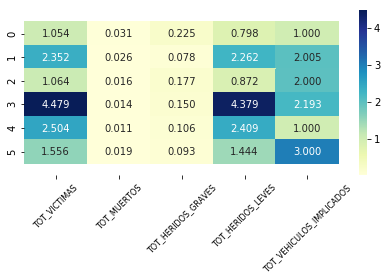
\includegraphics[width=120mm]{figures/accidentes/ward1centroids}
  \caption{Centroides de los clusters generados por Ward.}
  \label{fig:ward1centroids}
\end{figure}

\begin{figure}[H]
  \centering
  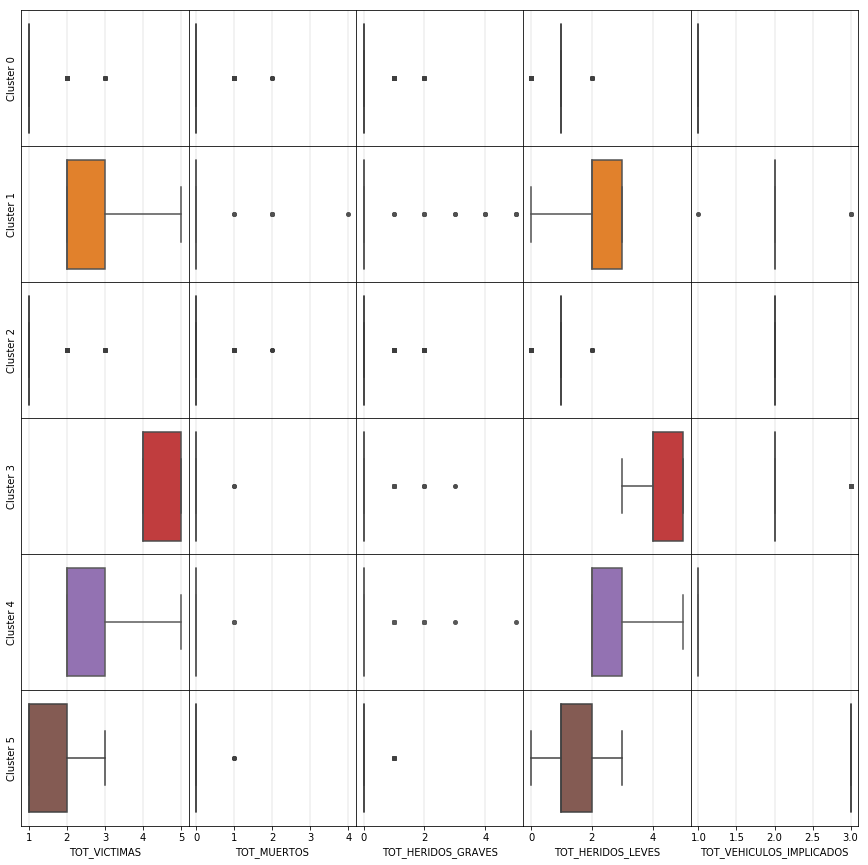
\includegraphics[width=125mm]{figures/accidentes/ward1distribution}
  \caption{Distribución de las variables en los clusters generados por
    Ward.}
  \label{fig:ward1distribution}
\end{figure}

Comprobamos que tampoco utiliza los muertos ni los heridos graves para
agrupar los clusters. Sí que hay algunas diferencias entre los valores
de estas variables en cada cluster, pero la inmensa mayoría presentan
el valor 0 y los considera como outliers (dentro del cluster). Por
tanto el número de cluster necesarios para tener una distinción en
estos atributos será mayor que 6 (al menos con este algoritmo). El
problema de esto es que los poco muertos y heridos graves se reparten
entre todos los clusters, aparecen algunos dentro de los clusters de
accidentes ``leves'' (con pocas víctimas, clusters 0 y 2), tratándose
claramente de excepciones e impurezas en la segmentación, lo que
también ocurre en el anterior agrupamiento.

Cada par de clusters se diferencian significativamente en el valor de
al menos una variable. Por ejemplo, los clusters 0 y 2 son muy
similares en cuanto a la distribución de valores de los atributos en
todas las variables salvo el total de vehículos implicados. Ambos
podrían costar de choques leves, pero los accidentes del cluster 2 (2
vehículos implicados) serían choques entre vehículos y los del cluster
0 (1 vehículo implicado) serían choques con obstáculos.

En la Figura \ref{fig:k-means1distribution} vimos que, exceptuando las
víctimas y heridos leves del cluster 0, cada atributo de cada cluster
presenta una distribución muy concentrada (sólo vemos una línea y
algunos puntos sueltos que considera outliers). En esta ocasión, los
atributos total de víctimas y total de heridos leves en los clusters
1, 3, 4 y 5 presentan distribuciones con rangos de valores más
amplios, ya que estos clusters son más pequeños y concentran
accidentes con diferentes rangos de valores de estas variables, no
centrados (de forma casi degenerada) en el valor 1.

Los clusters 1 y 4 son similares, contienen accidentes con dos o más
víctimas, la mayoría (como en todos los clusters) heridos leves. Se
diferencian principalmente en que los accidentes del cluster 1
acostumbran a tener dos vehículos implicados (podrían tratarse
colisiones entre vehículos con varios pasajeros de los cuales dos o
más resultan heridos), mientras que absolutamente todos los accidentes
del cluster 4 presentan un vehículo implicado (podrían tratarse de
colisones con obstáculos con varios pasajeros en el vehículo de los
cuales dos o más resultan heridos, y/o también atropellos múltiples).

El cluster 3 concentra los accidente con mayor número de heridos,
observamos que generalmente hay dos vehículos implicados, por lo que
podrían tratarse de choques fuertes frontales y laterales, los más
peligrosos.

El cluster 5 agrupa accidentes con exactamente 3 vehículos
implicados. Suelen presentar 1 o 2 víctimas, 3 en algunas ocasiones,
como podemos ver en la Figura \ref{fig:ward1distribution} abajo
(cluster 5) a la izquierda (total de víctimas). La mayoría de las
víctimas son leves, como ocurre en todos los clusters.

Además, teniendo en cuenta el tamaño de cada cluster observamos que
los accidentes leves con uno o dos vehículos implicados (clusters 0,
$\sim$36\% y 2, $\sim$37\% respectivamente) son los más comunes. Les
siguen accidentes algo más graves con dos vehículos implicados
(cluster 1, $\sim$13\%) o un solo vehículo implicado (cluster 4,
$\sim$6.4\%). Después el cluster 5 ($\sim$4\%) con accidentes con 3
vehículos implicados, y por último el cluster 3 ($\sim$3.4\%), con los
accidentes con mayor número de víctimas. Así nos hacemos una idea de
la frecuenca de cada tipo de accidente en las condiciones descritas en
el caso de estudio.

\textbf{Comparamos} finalmente \textbf{los scores de ambos
  algoritmos}.

\begin{table}[H]
  \centering
  \begin{tabular}{|l|ccc|} \hline & Calinski & Silhouette & $K$ \\
    \hline K-means & 4703.28 & 0.6437 & 3 \\ \hline Ward & 3925.91 &
    0.715 & 6 \\ \hline
  \end{tabular}
  \caption{Métricas Silhouette y Calinski para ambos agrupamientos.}
  \label{tab:comp-scores1}
\end{table}

K-means consigue mejor razón de Calinski, mientras que Ward consigue
un coeficiente Silhouette más alto. Por tanto, no tenemos en terminos
de score un claro ganador, aunque el agrupamiento que consigue K-means
ha sido más fácilmente interpretable debido al menor número de
clusters. El agrupamiento de Ward nos ha permitido formar grupos más
concretos de accidentes, pero quizá en algunos casos sean demasiado
concretos. Por ejemplo, los clusters 1, 2 y 3 constan de accidentes
con ǵeneralmente dos vehículos implicados, el cluster 2 agrupa los más
leves (menos heridos) y el cluster 3 los más graves (más heridos),
mientras que el cluster 1 estaría ``entre el 2 y el 3'', accidentes
graves pero no demasiado. Probablemente se podrían agrupar las
instancias del cluster 1 representando accidentes más leves en el
cluster 2 y fusionar el resto con el cluster 3, formando entonces un
cluster para accidentes leves con dos vehículos implicados y otro para
los más graves.

Si entre los 6 cluster generados por Ward hubiese uno o más que
agrupasen accidentes por muertos o heridos graves, sí que podría
compensar este aumento en el número de clusters generado. Aunque en
definitiva tenemos ya dos segmentaciones analizadas con distinto
número de clusters, por lo que se podría consultar una u otra según si
un problema requiere una segmentación con grupos más generales y
heterogéneos o más concretos y homogéneos.

\section{Caso de estudio 2: Análisis de los accidentes a altas horas
  de la madrugada frente a los ocurridos en horas puntas}

Nuestro segundo caso de estudio contrastará accidentes según la hora a
la que ocurren. En concreto distinguiremos dos clases de accidentes,
los ocurridos a altas horas de la noche y los ocurridos en horas
puntas. En el primer caso, tomamos accidentes ocurridos entre las 12
de la noche y las 6 de la madrugada. Horas en las que la gente suele
estar durmiendo, salvo transportistas de largas distancias
(conductores de camiones y trailers, por ejemplo), personas que
trabajan por la noche, personas que están en un viaje largo o que
salen de ocio nocturno, entre otros. Cabe esperar que en la mayoría de
estos accidentes (al menos los ocurridos a trabajadores) sólo vaya un
ocupante en el vehículo, y también que el accidente sea causado por
una distracción a causa del sueño o un exceso de confianza por la baja
densidad del tráfico. Esta última causa, además permitiría a los
conductores ``sentirse cómodos'' conduciendo a altas velocidades y
podría traducirse en un aumento en la gravedad de los accidentes.

En el segundo caso, tomaremos accidentes ocurridos en horas
puntas. Para ello, observaremos la distribución de accidentes respecto
a la hora en la que ocurren. Obtenemos este dato a partir del
DataFrame combinando los métodos \texttt{groupby} y \texttt{count}, y
consultando cualquier columna de la tabla:
\begin{verbatim}
n_accidentes=list(data.groupby('HORA').count().MES)
\end{verbatim}

\begin{figure}[H]
  \centering
  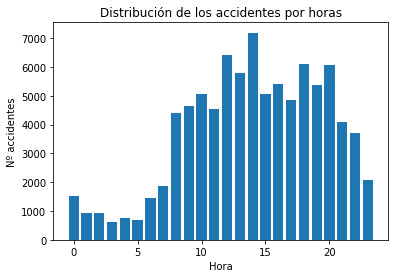
\includegraphics[width=120mm]{figures/accidentes/accidentes-hora}
  \caption{Distribución de accidentes por horas.}
  \label{fig:accidentes-hora}
\end{figure}

Hay varias horas puntas en las que ocurren mayor cantidad de
accidentes. Tomaremos dos horas puntas: las 14h (salida de los
colegios) y las 20h (salida de turnos de tarde).

En el primer caso, tenemos 5969 instancias. Comprobamos con
\texttt{Counter} que en esta ocasión hemos dejado fuera al accidente
con 52 víctimas, por lo que las escalas de los ejes no están demasiado
distorsionadas y no necesitamos limpiar los outliers (en la sección
\ref{sec:outliers} discutimos las consecuencias de eliminarlos).

\begin{figure}[H]
  \centering
  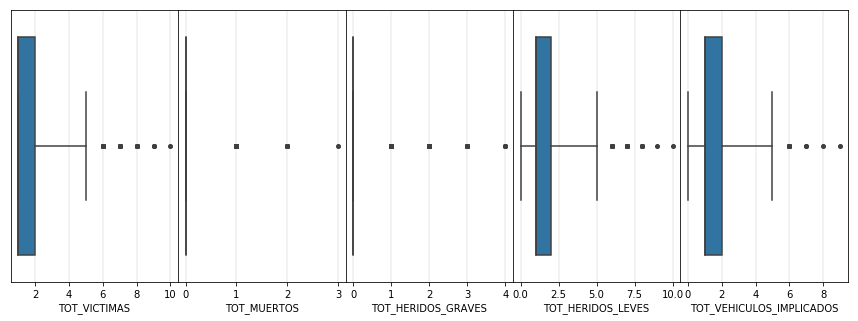
\includegraphics[width=160mm]{figures/accidentes/distrib-madrugada}
  \caption{Distribución de las variables en los accidentes a altas horas de la madrugada.}
  \label{fig:distrib-madrugada}
\end{figure}

En la segunda clase vuelve a aparecer el accidente con 52 víctimas, si
realizasemos una limpieza de outliers similar a la del primer caso de
estudio, tendríamos dificultades para comparar ambas clases por el
motivo que comentamos en la Sección \ref{sec:outliers}. Por tanto, lo
eliminamos con la siguiente línea de código:
\begin{verbatim}
data = data[data.TOT_VICTIMAS <=20]
\end{verbatim}
quedándonos con 6671 instancias. Observamos como varía la escala de
los ejes sólo con eliminar esta instancia.

\begin{figure}[H]
  \centering
  \subfigure[Antes de eliminar el outlier.]{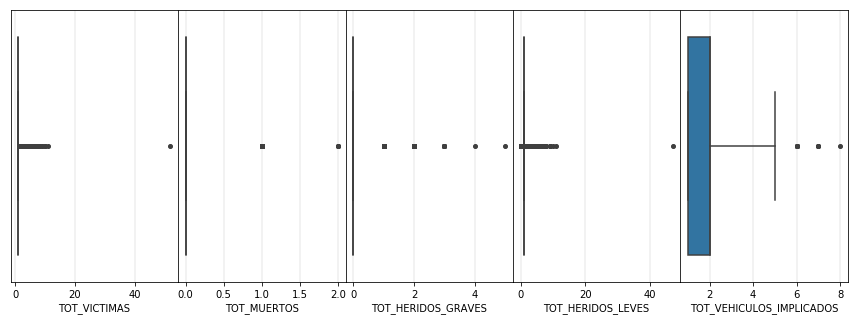
\includegraphics[width=160mm]{figures/accidentes/outliers2-1}}
  \subfigure[Tras eliminar el outlier.]{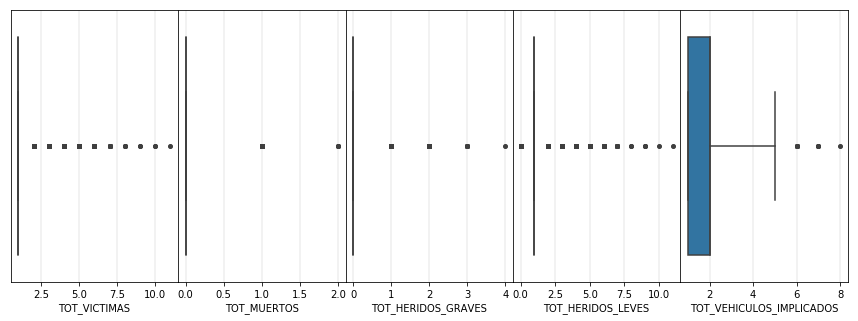
\includegraphics[width=160mm]{figures/accidentes/outliers2-2}}
  \caption{Distribución de las variables en los accidentes a horas
    puntas.}
  \label{fig:distrib-puntas}
\end{figure}

\subsection{Accidentes a altas horas de la madrugada}

\subsubsection{Algoritmos de clustering y resultados}

De nuevo comenzamos agrupando con \textbf{K-means}, seguimos el mismo
procedimiento que en la Sección \ref{sec:alg1} para determinar un
valor de $K$ adecuado. Obtenemos los siguientes resultados:

\begin{table}[H]
  \centering
\begin{tabular}{|c|cc|}
  \hline
  ~\hspace{2mm}K\hspace{2mm}~ & ~\hspace{2mm}Calinski\hspace{2mm}~ & ~\hspace{2mm}Silhouette\hspace{2mm}~ \\ \hline
2 & 3023.23 & 0.5977 \\ \hline
3 & 3620.77 & 0.6052 \\ \hline
4 & 3403.01 & 0.56 \\ \hline
5 & 3516.71 & 0.5981 \\ \hline
6 & 3796.63 & 0.7136 \\ \hline
7 & 3884.41 & 0.7199 \\ \hline
8 & 3916.43 & 0.7376 \\ \hline
9 & 4347.46 & 0.7777 \\ \hline
\end{tabular}
\caption{Scores de K-means para distinto número de clusters.}
\label{tab:k-means2}
\end{table}

\begin{figure}[H]
  \centering
  \subfigure[Razón de Calinski-Harabasz]{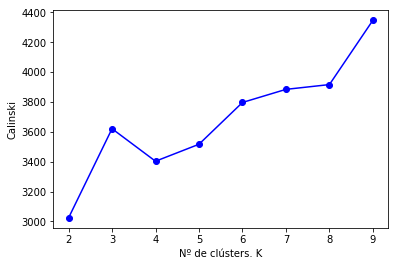
\includegraphics[width=87mm]{figures/accidentes/k-means2cal}}
  \subfigure[Coeficiente Silhouette]{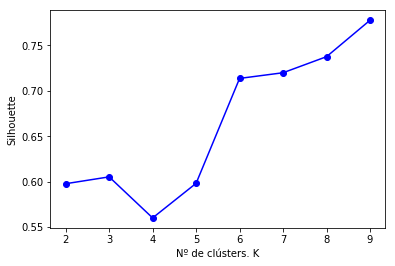
\includegraphics[width=87mm]{figures/accidentes/k-means2sil}}
  \caption{Representaciones de los scores de K-means para distinto número de clusters.}
  \label{fig:k-means2-scores}
\end{figure}

Observamos dos ganancias importantes de score, para $K=3$ en la razón
de Calinski y para $K=6$ en el coeficiente Silhouette. Analizaremos
los dos agrupamientos, pero no entraremos en tantos detalles como en
el caso anterior y nos centraremos en clusters especialmente
interesantes. Por ejemplo, si alguno agrupa accidentes por muertos y/o
por heridos graves.

Para $K=3$, obtenemos los siguientes tamaños de cluster:
\begin{verbatim}
Counter({0: 4652, 1: 717, 2: 600})
\end{verbatim}

Mientras que para $K=6$ obtenemos:
\begin{verbatim}
Counter({1: 2213, 5: 1399, 0: 1213, 4: 688, 2: 301, 3: 155})
\end{verbatim}

Esta vez el otro algoritmo que utilizaremos es
\href{https://scikit-learn.org/stable/modules/generated/sklearn.cluster.DBSCAN.html}{\textbf{DBSCAN}}. Los
dos parámetros que debemos proporcionarle son el radio máximo
(epsilon, $\varepsilon$) y el tamaño mínimo de cada cluster. En la
documentación de \textit{sklearn} explica que $\varepsilon$ es el
parámetro más influyente, por lo que fijaremos el tamaño mínimo a 50 y
probaremos varios valores de $\varepsilon$ (Figura
\ref{fig:dbscan1}). Observamos mucha diferencia entre los valores 0.1
y 0.15 tanto en Silhouette como en el número de clusters, así que
realizamos una segunda tanda de mediciones dentro de este intervalo.

En la segunda tanda de mediciones, descartamos 0.1 y 0.11 por producir
demasiados clusters. Los valores 0.12, 0.13 y 0.14 consiguen los
mismos scores porque producen las mismas particiones, la métrica
Calinski nos sugiere estos valores, pero tiene dos inconvenientes:
Generan un particionamiento con 8 clusters (sin contar el -1) y no son
capaces de agrupar 266 elementos (que los considera como ruidosos y
los concentra en el cluster -1). Tomaremos $\varepsilon=0.15$ porque
produce sólo 3 clusters y sólo desecha 183 instancias. 

\begin{table}[H]
  \centering
\begin{tabular}{|c|ccc|}
  \hline
   ~\hspace{2mm}$\varepsilon$\hspace{2mm}~ & ~\hspace{2mm}K\hspace{2mm}~ & ~\hspace{2mm}Calinski\hspace{2mm}~ & ~\hspace{2mm}Silhouette\hspace{2mm}~ \\ \hline
0.1 & 14 & 888.21 & 0.871 \\ \hline
0.15 & 3 & 1053.3 & 0.535 \\ \hline
0.2 & 4 & 848.14 & 0.5414 \\ \hline
0.25 & 4 & 862.67 & 0.5417 \\ \hline
0.3 & 2 & 358.65 & 0.526 \\ \hline
0.35 & 1 & 189.82 & 0.7647 \\ \hline
\end{tabular}
\quad
\begin{tabular}{|c|ccc|}
  \hline
   ~\hspace{2mm}$\varepsilon$\hspace{2mm}~ & ~\hspace{2mm}K\hspace{2mm}~ & ~\hspace{2mm}Calinski\hspace{2mm}~ & ~\hspace{2mm}Silhouette\hspace{2mm}~ \\ \hline
0.1 & 14 & 888.21 & 0.871 \\ \hline
0.11 & 14 & 888.21 & 0.871 \\ \hline
0.12 & 8 & 1540.86 & 0.59 \\ \hline
0.13 & 8 & 1540.86 & 0.59 \\ \hline
0.14 & 8 & 1540.86 & 0.59 \\ \hline
0.15 & 3 & 1053.3 & 0.535 \\ \hline
\end{tabular}
\caption{Scores de DBSCAN para distintos radios máximos de cluster.}
\label{tab:dbscan1}
\end{table}

\begin{figure}[H]
  \centering
  \subfigure{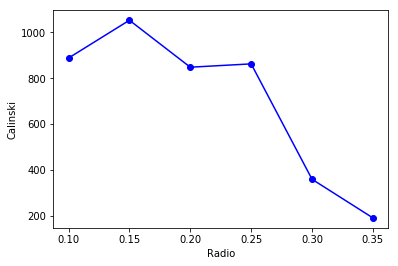
\includegraphics[width=57mm]{figures/accidentes/dbscan1cal}}
  \subfigure{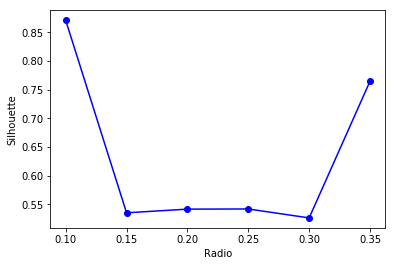
\includegraphics[width=57mm]{figures/accidentes/dbscan1sil}}
  \subfigure{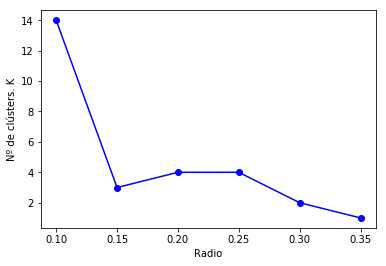
\includegraphics[width=57mm]{figures/accidentes/dbscan1k}}
  \subfigure{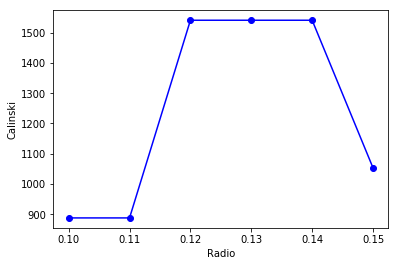
\includegraphics[width=57mm]{figures/accidentes/dbscan12cal}}
  \subfigure{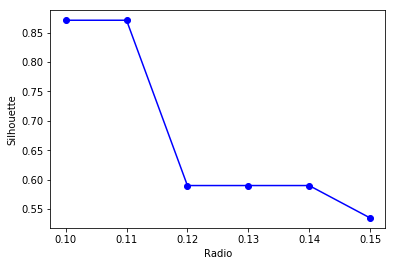
\includegraphics[width=57mm]{figures/accidentes/dbscan12sil}}
  \subfigure{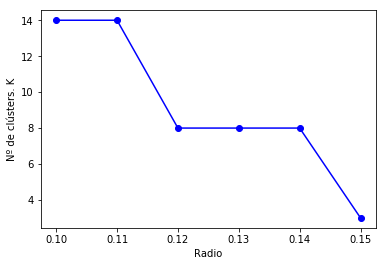
\includegraphics[width=57mm]{figures/accidentes/dbscan12k}}
  \caption{Scores y Nº de clusters de DBSCAN para distintos radios máximos.}
  \label{fig:dbscan1}
\end{figure}

Hay que tener en cuenta que este algoritmo agrupa los datos que
considera ruidosos en un único cluster con la etiqueta
-1. Desecharemos este cluster, por lo que perderemos algunas
instancias, en este caso 183. También vemos el tamaño del resto de
clusters.
\begin{verbatim}
Counter({-1: 183, 0: 5042, 1: 628, 2: 116})
\end{verbatim}
Desechamos el cluster -1 con el siguientes código, y también
aprovechamos para calcular los centroides a mano como hicimos con
Ward.
\begin{verbatim}
dataC=data.copy()
dataC['cluster']=labels
dataC.drop(dataC[dataC['cluster']==-1].index,inplace=True)
centroids = dataC.groupby('cluster').mean().values
\end{verbatim}

\subsubsection{Interpretación de la segmentación}

Representamos primero para $K=3$ los centroides y distribuciones de
cada cluster.

\begin{figure}[H]
  \centering
  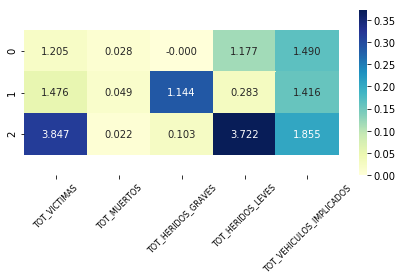
\includegraphics[width=92mm]{figures/accidentes/k-means2centroids}
  \caption{Centroides de los clusters generados por K-means.}
  \label{fig:k-means2centroids}
\end{figure}

\begin{figure}[H]
  \centering
  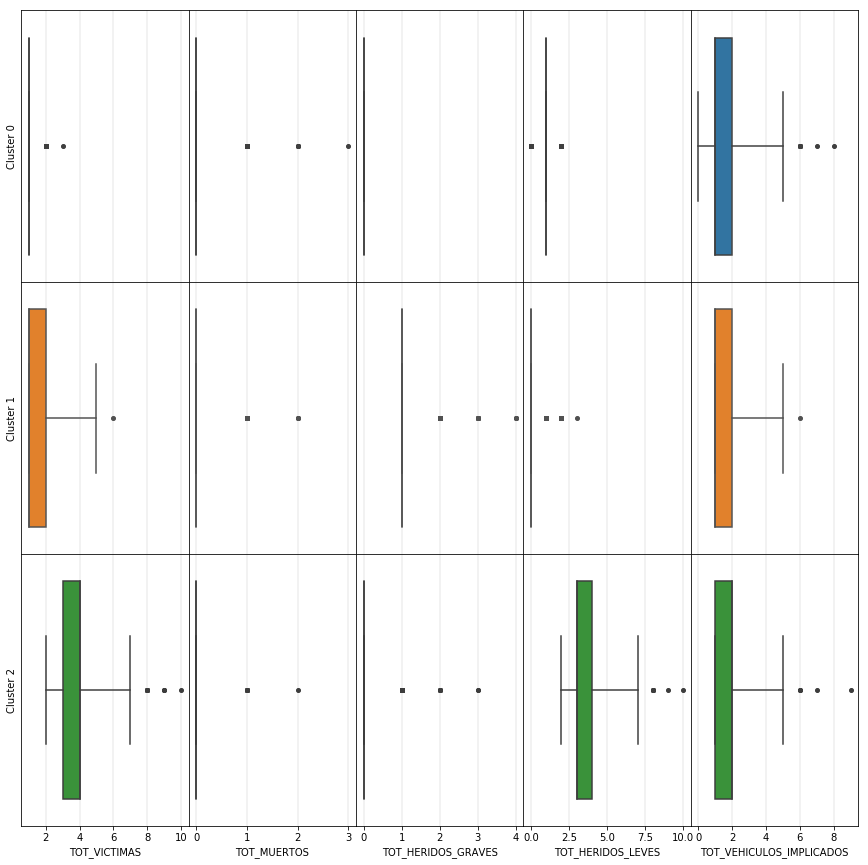
\includegraphics[width=140mm]{figures/accidentes/k-means2distribution}
  \caption{Distribución de las variables en los clusters generados por
    K-means.}
  \label{fig:k-means2distribution}
\end{figure}

Observamos que el número de vehículos implicados no se utiliza para
distinguir clusters. Tenemos el cluster 0 (mucho más grande) con
accidentes leves, el cluster 2 con accidentes con un elevado número de
víctimas (la mayoría leves) y el cluster 1, que agrupa los accidentes
con heridos graves.

El número de muertos sigue sin ser lo suficientemente significativo
para que se tenga en cuenta en esta segmentación, pero por primera vez
observamos un cluster que agrupa accidentes con heridos graves.

Esta vez los 5969 accidentes acumulan 180 muertos y 882 heridos
graves. En cuanto a muertos, es una proporción más grande que en el
primer caso de estudio. Mientras que en cuanto a heridos graves es una
proporción similar.

Al igual que en el anterior caso de estudio, la mayoría de las
víctimas son leves. Pero en este uno de los problemas que comentamos
en pairplot (no se distinguía si había un accidente o 1000 con
determinados valores de las variables, simplemente aparecía un punto)
no nos impide visualizarlo. En la Figura \ref{fig:k-means2pair},
observamos que las gráficas que comparan el número de víctimas con el
número de heridos leves tienen aproximadamente una tendencia lineal
con pendiente 1, esto significa que el número de heridos leves es casi
el número de víctimas. Obviamente no puede haber más heridos leves que
víctimas, puesto que
\[\text{TOT\_VICTIMAS=TOT\_MUERTOS+TOT\_HERIDOS\_GRAVES+TOT\_HERIDOS\_LEVES}\]
El cluster 1 (puntos naranjas) es una excepción a esta tendencia,
puesto que agrupa los accidentes con heridos graves.

Esta tendencia lineal entre el número de víctimas y heridos leves se
observa en el resto de pairplots de este caso de uso para todas las
segmentaciones, tanto con los accidentes a altas horas de la madrugada
como con los accidentes en horas puntas. Así que omitiremos el resto
de pairplots.

También en la Figura \ref{fig:k-means2pair}, en la gráfica de la
diagonal correspondiente a los heridos graves observamos que los
elemenos del cluster 1 concentran la mayoría de accidentes con heridos
graves, exceptuando algunos accidentes sueltos que están en el cluster
2, probablemente porque presenten un elevado número de víctimas. En la
Figura \ref{fig:k-means2distribution} se observa que el cluster 0 no
presenta un sólo accidente con heridos graves, por lo que no aparece
(no se representan distribuciones degeneradas, salta un warning de
varianza 0).

\begin{figure}[H]
  \centering
  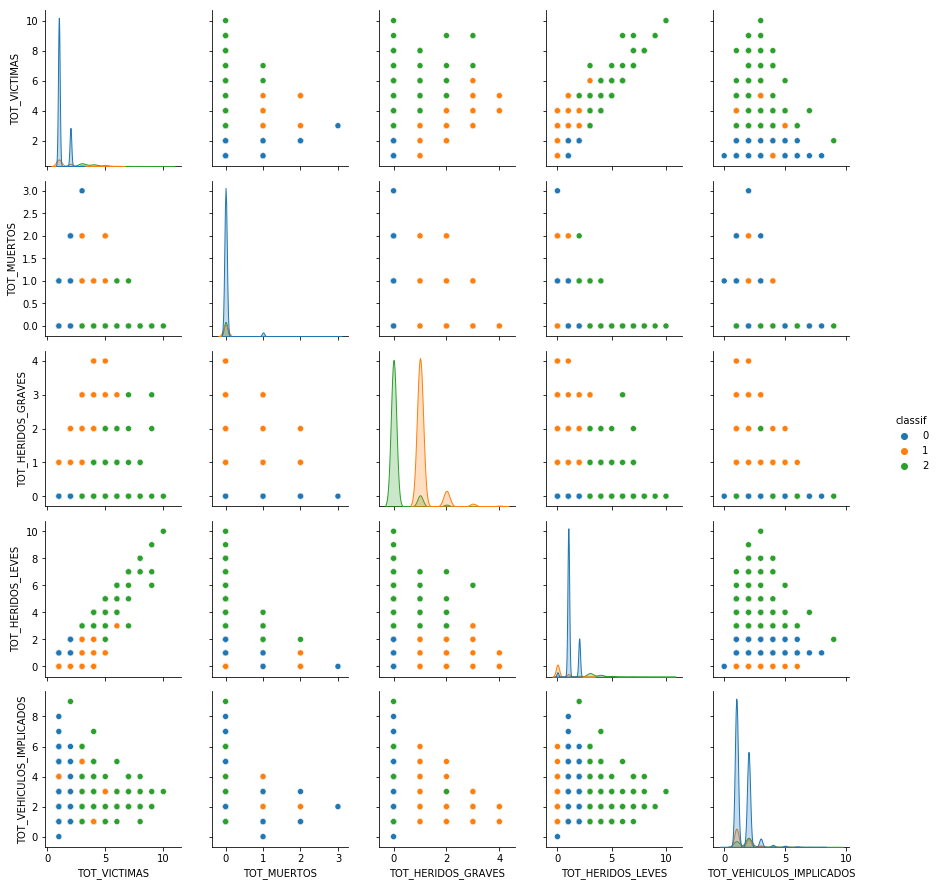
\includegraphics[width=160mm]{figures/accidentes/k-means2pair}
  \caption{Pairplot del agrupamiento generado por K-means para $K=3$.}
  \label{fig:k-means2pair}
\end{figure}

\pagebreak

Para $K=6$ generamos las representaciones análogas:

\begin{figure}[H]
  \centering
  \includegraphics[width=100mm]{figures/accidentes/k-means22centroids}
  \caption{Centroides de los clusters generados por K-means.}
  \label{fig:k-means22centroids}
\end{figure}

\begin{figure}[H]
  \centering
  \includegraphics[width=135mm]{figures/accidentes/k-means22distribution}
  \caption{Distribución de las variables en los clusters generados por
    K-means.}
  \label{fig:k-means22distribution}
\end{figure}

Esta vez tenemos por fin un cluster que agrupa por muertos (cluster 3)
y otro que agrupa por heridos graves (cluster 4). Como consecuencia,
el resto de cluster apenas presentan muertos, sólo hay algunos
accidentes con muertos en los cluster 2 (porque presentará un elevado
número de víctimas) y en cluster 4 (porque también habrá heridos
graves).

En la segmentación con \textbf{DBSCAN} tenemos las siguientes representaciones:

\begin{figure}[H]
  \centering
  \includegraphics[width=100mm]{figures/accidentes/dbscan1centroids}
  \caption{Centroides de los clusters generados por DBSCAN.}
  \label{fig:dbscan1centroids}
\end{figure}

\begin{figure}[H]
  \centering
  \includegraphics[width=120mm]{figures/accidentes/dbscan1distribution}
  \caption{Distribución de las variables en los clusters generados por
    DBSCAN.}
  \label{fig:dbscan1distribution}
\end{figure}

Esta vez se han utilizado únicamente los muertos y heridos graves para
la segmentación. El cluster 0 incluye accidentes donde todos los
heridos son leves. El cluster 1 incluye accidentes donde hay un único
herido grave y ningún muerto. Y el cluster 2 incluye accidentes donde
hay un único muerto y ningún herido grave. Podemos observar en la
figura \ref{fig:dbscan1distribution} que no hay excepciones a esta
regla, esto se debe a que los accidentes con más de un muerto, más de
un herido grave o tanto muertos como heridos graves han sido agrupados
con los outliers y descartados en el cluster -1.

No se ha utilizado el número de víctimas ni de vehículos implicados
para el agrupamiento, pero podemos observar en la figura
\ref{fig:dbscan1centroids} que los accidentes con mayor gravedad (con
muertos, seguidos de con heridos graves) acostumbran a presentar un
menor número de vehículos implicados y menor número de víctimas
totales. Aunque tenemos que interpretar esto con cuidado, pues el
número de elementos en el cluster 2 (116) es menor que el del cluster
-1 (183). Por tanto, esas 183 instancias que el algoritmo ha dejado
sin agrupar podrían cambiar drásticamente esta tendencia.

\subsection{Accidentes a horas puntas}

\subsubsection{Algoritmos de clustering y resultados}

Una vez más, buscamos un $K$ adecuado para \textbf{K-means}, probamos
valores y obtenemos los siguientes scores:

\begin{table}[H]
  \centering
\begin{tabular}{|c|cc|}
  \hline
  ~\hspace{2mm}K\hspace{2mm}~ & ~\hspace{2mm}Calinski\hspace{2mm}~ & ~\hspace{2mm}Silhouette\hspace{2mm}~ \\ \hline
2 & 2696.34 & 0.6136 \\ \hline
3 & 3042.18 & 0.6097 \\ \hline
4 & 3856.17 & 0.6435 \\ \hline
5 & 3842.02 & 0.7095 \\ \hline
6 & 4015.9 & 0.7259 \\ \hline
7 & 4439.09 & 0.7731 \\ \hline
8 & 4621.84 & 0.805 \\ \hline
9 & 4772.9 & 0.8667 \\ \hline
\end{tabular}
\caption{Scores de K-means para distinto número de clusters.}
\label{tab:k-means22}
\end{table}

\begin{figure}[H]
  \centering
  \subfigure[Razón de Calinski-Harabasz]{\includegraphics[width=87mm]{figures/accidentes/k-means22cal}}
  \subfigure[Coeficiente Silhouette]{\includegraphics[width=87mm]{figures/accidentes/k-means22sil}}
  \caption{Representaciones de los scores de K-means para distinto número de clusters.}
  \label{fig:k-means22-scores}
\end{figure}

Observando las gráficas, Calinski nos sugiere $K=4$ y Silhouette
$K=5$. Elegimos $K=4$ para que la segmentación sea más fácilemente
interpretable. Obtenemos los siguientes tamaños de cluster:
\begin{verbatim}
Counter({0: 3629, 1: 497, 2: 2020, 3: 525})
\end{verbatim}

Hacemos lo mismo con \textbf{DBSCAN} para estimar un radio adecuado.

\begin{table}[H]
  \centering
\begin{tabular}{|c|ccc|}
  \hline
   ~\hspace{2mm}$\varepsilon$\hspace{2mm}~ & ~\hspace{2mm}K\hspace{2mm}~ & ~\hspace{2mm}Calinski\hspace{2mm}~ & ~\hspace{2mm}Silhouette\hspace{2mm}~ \\ \hline
0.1 & 10 & 1217.9 & 0.8902 \\ \hline
0.15 & 2 & 1071.13 & 0.5441 \\ \hline
0.2 & 2 & 1024.81 & 0.5426 \\ \hline
0.25 & 2 & 1024.81 & 0.5426 \\ \hline
0.3 & 1 & 445.16 & 0.7473 \\ \hline
0.35 & 1 & 449.2 & 0.7369 \\ \hline
\end{tabular}
\quad
\begin{tabular}{|c|ccc|}
  \hline
   ~\hspace{2mm}$\varepsilon$\hspace{2mm}~ & ~\hspace{2mm}K\hspace{2mm}~ & ~\hspace{2mm}Calinski\hspace{2mm}~ & ~\hspace{2mm}Silhouette\hspace{2mm}~ \\ \hline
0.1 & 10 & 1217.9 & 0.8902 \\ \hline
0.11 & 10 & 1217.9 & 0.8902 \\ \hline
0.12 & 10 & 1217.9 & 0.8902 \\ \hline
0.13 & 10 & 1217.9 & 0.8902 \\ \hline
0.14 & 6 & 1111.97 & 0.6051 \\ \hline
0.15 & 2 & 1071.13 & 0.5441 \\ \hline
\end{tabular}
\caption{Scores de DBSCAN para distintos radios máximos de cluster.}
\label{tab:dbscan2}
\end{table}

\begin{figure}[H]
  \centering
  \subfigure{\includegraphics[width=57mm]{figures/accidentes/dbscan2cal}}
  \subfigure{\includegraphics[width=57mm]{figures/accidentes/dbscan2sil}}
  \subfigure{\includegraphics[width=57mm]{figures/accidentes/dbscan2k}}
  \subfigure{\includegraphics[width=57mm]{figures/accidentes/dbscan22cal}}
  \subfigure{\includegraphics[width=57mm]{figures/accidentes/dbscan22sil}}
  \subfigure{\includegraphics[width=57mm]{figures/accidentes/dbscan22k}}
  \caption{Scores y Nº de clusters de DBSCAN para distintos radios máximos.}
  \label{fig:dbscan2}
\end{figure}

Nos ha vuelto a ocurrir lo mismo, había mucha diferencia en Silhouette
y en el número de clusters entre $\varepsilon=0.1$ y
$\varepsilon=0.15$. Por lo que volvemos a evaluar las métricas para
varios valores de ese intervalo. Nos quedaremos con
$\varepsilon=0.15$, que genera menos clusters (2 frente a 6), agrupa
menos elementos en el cluster -1 (124 frente a 170) y la diferencia en
las métricas no es demasiada. Obtenemos los siguientes tamaños de
cluster, y descartaremos el cluster -1.
\begin{verbatim}
Counter({-1: 124, 0: 6074, 1: 473})
\end{verbatim}

\subsubsection{Interpretación de la segmentación}

Visualizamos los centroides y la distribución los valores de los
atributos en cada cluster para el agrupamiento generado por
\textbf{K-means}.

\begin{figure}[H]
  \centering
  \includegraphics[width=120mm]{figures/accidentes/k-means3centroids}
  \caption{Centroides de los clusters generados por K-means.}
  \label{fig:k-means3centroids}
\end{figure}

\begin{figure}[H]
  \centering
  \includegraphics[width=130mm]{figures/accidentes/k-means3distribution}
  \caption{Distribución de las variables en los clusters generados por
    K-means.}
  \label{fig:k-means3distribution}
\end{figure}

Observamos dos clusters de accidentes leves (normalmente un sólo
herido leve), uno con exactamente (en la Figura
\ref{fig:k-means3distribution} se ve una barra en el 1 y ningún punto
en el resto de valores) un vehículo implicado (cluster 2) y el otro
con dos o más (cluster 0). Otro cluster (cluster 1) con accidentes con
más víctimas, aunque la mayoría leves. El cluster 3 agrupa los
accidentes con heridos graves.

En esta ocasión, el agrupamiento tampoco diferencia por el total de
muertos, probablemente por el reducido número de muertos en estos
accidentes. Entre los 6671 accidentes suman 47 muertos, la proporción
más baja entre las clases que hemos estudiado.

Ahora analizamos el agrupamiento generado por \textbf{DBSCAN}:

\begin{figure}[H]
  \centering
  \includegraphics[width=110mm]{figures/accidentes/dbscan3centroids}
  \caption{Centroides de los clusters generados por DBSCAN.}
  \label{fig:dbscan3centroids}
\end{figure}

\begin{figure}[H]
  \centering
  \includegraphics[width=140mm]{figures/accidentes/dbscan3distribution}
  \caption{Distribución de las variables en los clusters generados por
    DBSCAN.}
  \label{fig:dbscan3distribution}
\end{figure}

Tenemos el cluster 0, mucho más numeroso, que agrupa los accidentes
sin heridos leves. Mientras que el cluster 1, más reducido, agrupa los
accidentes con un único herido grave. En la Figura
\ref{fig:dbscan3distribution} observamos que no hay excepciones.

Entre los 124 datos que DBSCAN considera como ruidosos y agrupa en el
cluster -1, están todos los accidentes con víctimas mortales y los que
tienen más de un herido grave. Por la baja proporción de este tipo de
accidentes dentro de la clase, el algoritmo los ha considerado como
ruidosos.

\subsection{Comparación de ambas clases}

Compararemos las dos clases que acabamos de segmentar. Intuitivamente,
los accidentes a altas horas de la noche deberían producirse en calles
o carreteras prácticamente vacías, donde la gente suele conducir muy
rápido, a la máxima velocidad permitida por la vía y en ocasiones
sobrepasando el límite. Esto se traduciría en accidentes graves.

Los accidentes a horas puntas deberían producirse en el interior de
las ciudades y en circunvalaciones, con tráfico denso o colapsado,
donde la gente va más atenta y despacio. Según esta intuición deberían
de ser accidentes más leves, como choques suaves o por alcance en el
caso de atascos o semáforos.

Atenderemos a los agrupamientos generados por K-means. En la clase de
accidentes a altas horas de la madrugada tenemos 5969 instancias. El
agrupamiento con $K=3$ (figuras \ref{fig:k-means2centroids} y
\ref{fig:k-means2distribution}) nos proporcina los siguientes
clusters:
\begin{enumerate}\setcounter{enumi}{-1}
\item 4652 instancias. Accidentes con normalmente un herido leve y sin
  heridos graves ni muertos. Generalmente 1 o 2 vehículos
  implicados.
\item 717 instancias. Accidentes con al menos un herido grave (la
  mayoría tienen 1), normalmente no tienen heridos leves (salvo alguna
  excepción).
\item 600 instancias. Accidentes con dos o más víctimas, la mayoría de
  ellas leves. Aunque la mayoría de accidentes de este cluster
  presentan 3 ó 4 víctimas.
\end{enumerate}

En la clase de accidentes a horas puntas tenemos 6671 instancias. El
agrupamiento con $K=4$ (figuras \ref{fig:k-means3centroids} y
\ref{fig:k-means3distribution}) nos proporciona los siguientes
clusters:
\begin{enumerate}\setcounter{enumi}{-1}
\item 3629 instancias. Accidentes con normalmente un herido leve y sin
  heridos graves ni muertos, con 2 o más vehículos implicados
  (generalmente dos).
\item 497 instancias. Accidentes con dos o más víctimas, la mayoría de
  ellas leves. Aunque la mayoría de accidentes de este cluster
  presentan 3 ó 4 víctimas.
\item 2020 instancias. Accidentes con normalmente un herido leve y sin
  heridos graves ni muertos, con exactamente un vehículo implicado.  
\item 525 instancias. Accidentes con al menos un herido grave (la
  mayoría tienen 1), normalmente no tienen heridos leves (salvo alguna
  excepción). 
\end{enumerate}

Parece que los agrupamientos son similares y que el cluster 0 de la
primera clase equivale a los clusters 0 y 2 de la segunda. Estos
accidentes más leves (una sola víctima y leve) representan un 77.936\%
de los accidentes en la primera clase (madrugada) y un 84.68\% de los
accidentes en la segunda (horas puntas).

El cluster 1 de la primera clase equivale al cluster 3 de la segunda
clase. Estos accidentes con heridos graves representan un 12\% en la
primera clase y un 7.87\% en la segunda.

El cluster 2 de la primera clase equivale al cluster 1 de la
segunda. Estos accidentes con múltiples víctimas (la mayoría leves)
representan un 10.05\% de los accidentes de la primera clase y un
7.45\% de los de la segunda.

Estos dos últimos párrafos describen dos clases de accidentes de mayor
gravedad, ya sea por número de heridos o por gravedad de los
heridos. Entre los accidentes a altas horas de la madrugada, estos más
graves representan un porcentaje mayor que en los accidentes en horas
puntas, donde la proporción de accidentes con sólo un herido leve es
mayor. Esto apoya nuestra intuición de que los accidentes a horas
puntas son más leves que los accidentes a altas horas de la madrugada.

\section{Contenido adicional}

\subsection{Outliers y la poca importancia de los heridos graves y
  muertos} \label{sec:outliers}

Hemos observado que en el primer caso de uso ninguno de los algoritmos
ha distinguido por heridos graves ni muertos a la hora de generar los
clusters. Los 4143 datos del caso de estudio 1 suman 92 muertos y 714
heridos graves, que en proporción es mayor a los 595 heridos graves y
47 muertos que acumulan los 6671 accidentes ocurridos a horas puntas,
donde sí se ha utilizado el atributo total de heridos graves para la
segmentación.

Este problema genera impurezas en los clusters, por ejemplo un
accidente con un sola víctima que muere o resulta herida grave (un
atropello, por ejemplo) podría aparecerer en el cluster de los
accidentes leves (un sola víctima, que normalmente es leve), por el
hecho de presentar una sóla víctima. Cuando, de no agrupar por heridos
graves y muertos, quizá tuviese más sentido agrupar ese accidente en
un cluster de accidentes con múltiples víctimas, que podemos
considerar accidentes más graves.

El origen de este problema se debe a que hemos tomado la decisión de
limpiar los datos de outliers en el resto de atributos (número de
víctimas, heridos leves y vehículos implicados). Esto provoca que al
normalizar los atributos entre 0 y 1, los atributos en los que
limpiamos los outliers ganen más relevancia.

Por ejemplo, en presencia del accidente con 52 víctimas. Al normalizar
con \texttt{MinMaxScaler}, los accidentes con 5 víctimas obtienen el
valor $\frac{5-1}{52-1}\approx 0.078$. Mientras que si el máximo de
víctimas fuese 10, este valor sería de $\frac{5-1}{10-1}\approx
0.44$. Si el número máximo de muertos es 4, un accidente con un muerto
pasaría a tener el valor $\frac{1}{4}=0.25$. En el primer caso (sin
limpiar outliers), se considerarían dos accidentes con el mismo número
de muertos pero que se diferencien en 5 víctimas más similares que dos
accidentes que se diferencien en 1 muerto pero en menos de 5
víctimas. En el segundo caso (limpiando outliers), ocurre lo
contrario.

Esto se podría solucionar de diversas formas, al menos para el
agrupamiento con $K=6$:
\begin{itemize}
\item Crear una métrica customizada en lugar de la euclídea que
  utilizan por defecto los algoritmos para dar más peso a estas
  variables.
\item No limpiar los outliers, al coste de que las gráficas tengan
  ejes con escalas desproporcionadas. En presencia de un accidente con
  52 víctimas, no podríamos distinguir entre 1 víctima y 4 víctimas
  con un simple vistazo a la gráfica, ya que se verían muy próximos.
\item Haber limpiado también los outliers en los atributos número de
  muertos y de heridos graves. El problema de esta medida es que
  tomando $\mu\pm 3\cdot\sigma$ como margen (normalmente se utiliza
  1.5 en lugar de 3), se eliminaban todos los muertos y heridos
  graves. Podríamos haber tomado más margen, o simplemente haber
  colapsado en 1 ó 2 los valores de estos atributos que los superasen,
  de forma que los atributos número de muertos y heridos graves
  pierdan menos importancia al normalizar.
\item Haber limpiado los outliers manualmente. Esto no siempre es
  posible, pero es lo que hemos aplicado en el segundo caso de estudio
  eliminando solamente el accidente con 52 víctimas.
\end{itemize}

\subsection{Estudio de variables circunstanciales y de tipo dentro de
  los clusters}

En la interpretación del agrupamiento por K-menas del primer caso de
uso (figuras \ref{fig:k-means1centroids} y
\ref{fig:k-means1distribution}), especulamos con los tipos de
accidentes que podrían formar cada cluster. Comprobaremos si estábamos
en lo cierto. TODO

\section{Bibliografía/Webgrafía}

\end{document}
